%\clearpage
\section{Models}
\label{sec:models}

In this section, several canonical as well as recently proposed models
are presented. Modelling is divided into three categories: purely
temporal modelling, spatial modelling and spatio-temporal modelling.
 
\subsection{Temporal Modelling}
\label{ssec:temporal_modelling}

Purely temporal models only focus on the time series properties of the
traffic matrix. A key application of these models is in anomaly
detection, so as to be able to pinpoint the time and location of the
anomalous event. This is especially vital in detecting attacks on the
network or worm outbreaks. However, temporal behaviour is also
important in prediction, say for planning capacity of a future
network.

Before delving into the models, some basic issues regarding the
temporal properties of OD flows need to be understood. It is commonly
agreed that IP data traffic is rising exponentially, and has been for
more than a 
decade~\cite{claffy94:_track_long_term_growt_of_nsfnet,groschwitz94:_time_series_model_of_long,odlyzko03:_internet_growth,cisco_visual_networ_index2011}. There
was much early controversy about such growth estimates, because the
growth rate was vastly overestimated based on a small sample of
data. However, these days, exponential growth is considered the common
case (though with a much lower rate of growth), and is justified both
by data, and as a consequence of increasing computational and
networking speeds, governed by Moore's and Gilder's laws
respectively. As of the present, the introduction of mobile devices
and the rapid growth of traffic from these devices are set to further
increase data traffic in the years to come. Cisco (who admittedly have
a vested interest in a high forecast) estimate that ``Annual global IP
traffic will surpass the zettabyte threshold (1.3 zettabytes) by the
end of 2016''~\cite{cisco_visual_networ_index2011}.

Relatively few countries appear to monitor their national traffic, but
Australia is an exception. The Australian Bureau of Statistics have
collected and published traffic statistics for many
years~\cite{13:_abs_internet}. \autoref{fig:aust_traffic} shows the
growth of traffic in Australia from 2000 to 2012.
 
\begin{figure}[!b]
  \begin{center}
    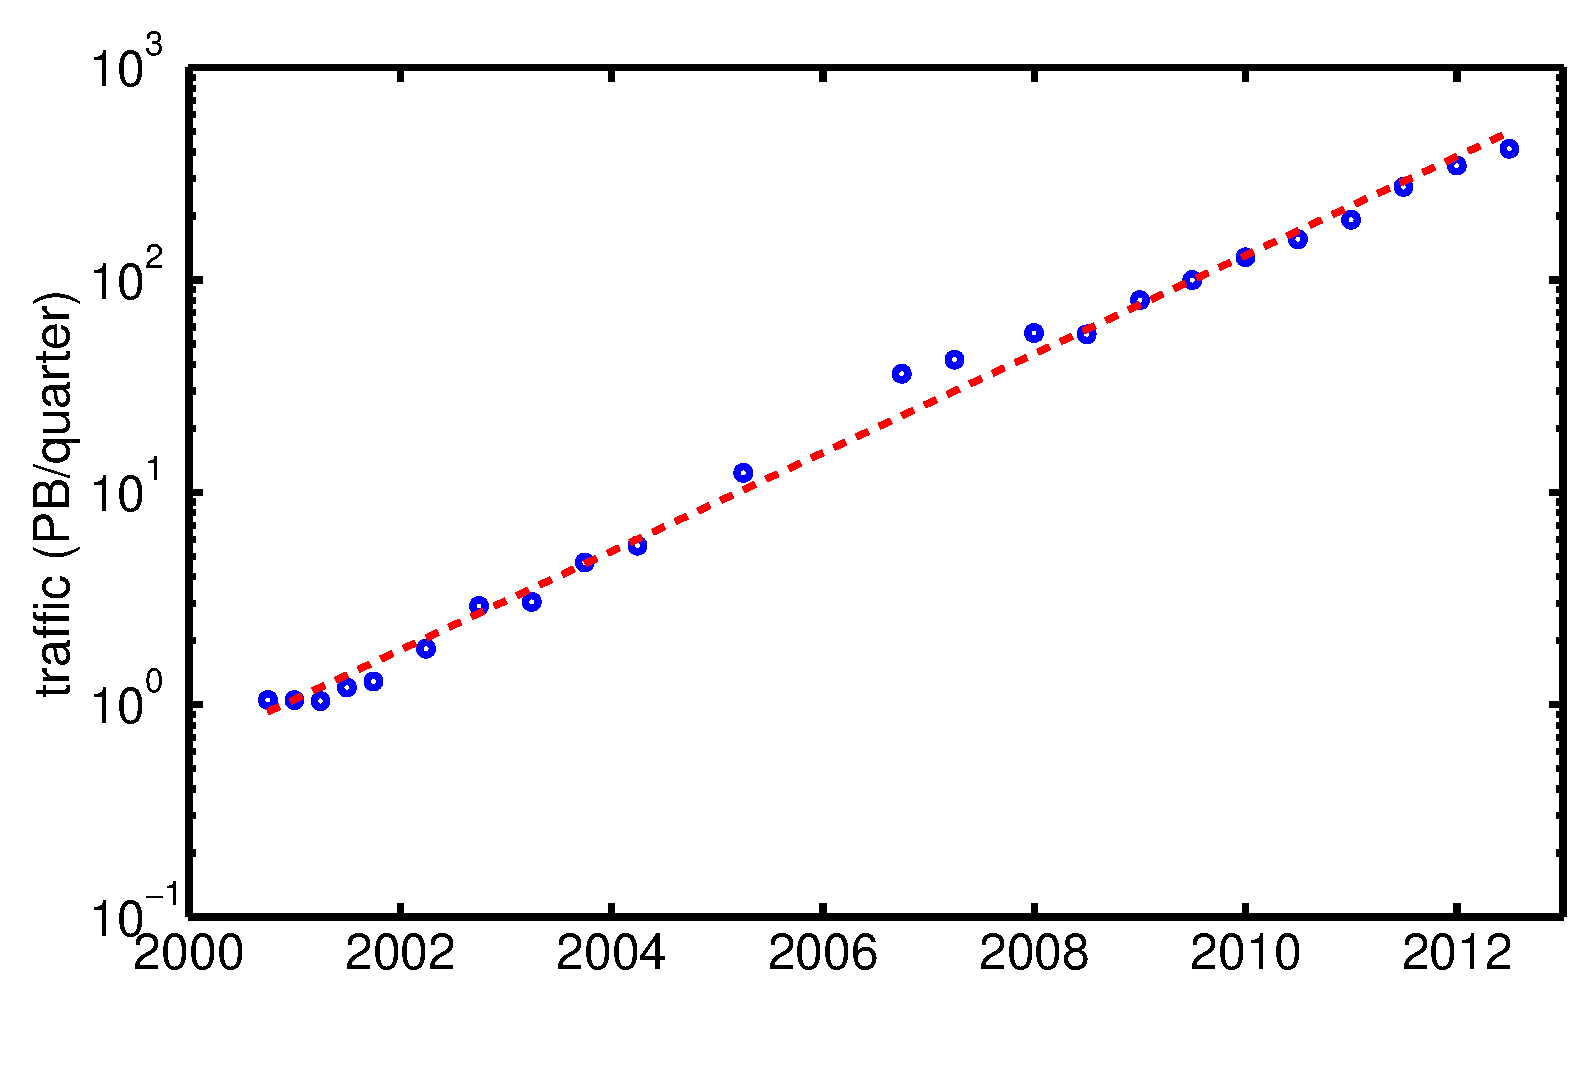
\includegraphics[width=0.7\oneup]{australian_internet_usage_log.eps}
    \caption{Australian Internet traffic volumes based on data from
      the Australian Bureau of Statistics from 2000-2012. The
      dashed line shows a linear fit to the (log) data.  Note
      the log $y$-axis, so the plot shows quite a reasonable fit to
      exponential growth with a doubling period of 465 days. Over the
      same period the growth in broadband subscribers has been almost
      exactly linear (soon this trend must decrease as a large
      proportion of Australia's population are now connected), so most of
      the growth has come from growth in the amount downloaded per customer.
      \label{fig:aust_traffic}}
  \end{center}
\end{figure}

Regardless of your belief about the rate of growth, and/or the best
model (exponential is common, but linear and logistic models may also
be appropriate in many cases), any model of long-term traffic needs to
be able to incorporate such growth.

Second, most network traffic is human generated. Therefore, it stands
to reason that traffic is influenced by human activity in a 24 hour
cycle. In fact, distinct diurnal patterns have been observed, with
peak traffic occurring around mid-day or in the evening and dips
during the night, for example see \autoref{fig:abilene_2004_b}. This
correlates to the daily schedule of an average human being, where
mid-day traffic is generated for work or school purposes, while the
lack of traffic during the night correlates to sleeping periods.  Peak
traffic rate is also noticeably less on the weekends.  The regularity
of this behaviour can be quite strong as shown in the figure where two
successive weeks' data are overlaid so one can see how closely they
match. Most traffic measurements see some measure of cyclic behaviour,
with the degree of regularity determined by the type of traffic (is it
made up of many individuals or a few large flows) and the scale.

% \begin{figure}[thbp] 
%   \begin{center}
%     \hfill
%     \begin{subfigure}[b]{\twoup}
%       \centering
%       \Diurnal
%       \caption{Traffic rate over the span of a single week starting
%         from May 7th, 2001, with the traffic rate of
%         the following week overlaid.}
%       \label{fig:cycle_week}
%     \end{subfigure}
%     \hfill
%     \begin{subfigure}[b]{\twoup}
%       \centering
%       \DiurnalZoom
%       \caption{Traffic rate of a single day,  May 8th
%         2001, on the same ISP, with traffic on  
%         May 15th, 2001 overlaid on top.}
%       \label{fig:cycle_day}
%     \end{subfigure}  
%     \hfill\mbox{ } \\
    
%     \caption{Observations of the cyclicality of the total traffic rate of a large PoP.\label{fig:cycle}}
%   \end{center}
% \end{figure}         


Third, and leading from the last point, the traffic volume itself is
dependent on the measurement period and the aggregation level of
traffic. At very short scales, in milli-seconds or seconds, the
traffic distribution is highly variable, and shows strong
dependencies, making use of such measures statistically non-trivial,
even if such measurements were easy to collect.  A common paradigm is
to consider a measurement interval of minutes to an hour, where
measurement is easy. Also important is the fact that at these times
scales \emph{stationarity}\footnote{Stationarity refers to the concept
  that the statistics of the traffic (for instance, the mean and
  variance, but in general including all statistics) are constant with
  respect to the time at which they are measured. Wide-sense
  stationarity is when only the mean and variance of the traffic
  satisfies the stationarity property.  In Internet traffic data it is
  only ever approximately true.  Moreover, it is hard to test for
  stationarity when traffic has long-term correlations, and so we can
  only ever talk about the degree of stationarity.} of the traffic
volume distribution is often a reasonable assumption, though we can
see the limits of this in \autoref{fig:abilene_2004_b} (stationarity clearly
doesn't hold for more than a couple of hours), however it was shown
that {\em cyclo-stationarity} holds to a large extent
\cite{Soule04TMLargest}.

Fourth, there are natural variations in traffic over time, and these
are often modelled as a random (or stochastic) process. This random
process could have all sorts of features, but there are some basics
that should be observed by all reasonable models. For instance,
network operators aggregate traffic from multiple sources, which is
known as \emph{multiplexing}. Multiplexing is used to boost the
efficiency of the links in a network by ``smoothing'' out variations
in traffic. The apparent smoothness is a result of decreases in the
relative variance, as predicted by the central limit
theorem~\cite{Cao01Nonstationarity}.  The more OD flows multiplexed on a
link, the higher the efficiency and smoothing effect, provided the
aggregated bandwidth does not exceed link capacity. Thus, any model
for the large traffic rates in a network must be consistent under
multiplexing, for example, when the number of flows being multiplexed
is increased the relative variance should decrease in a predictable
manner. Furthermore, the statistical properties of the aggregated
traffic must also be consistent with the statistical assumptions of
the traffic from a single user.

Finally, although rare, sometimes there may be sudden ``spikes'' in
traffic.  Such a component may arise from unusual traffic behaviour,
such as DDoS attacks, worm propagation or Border Gateway Protocol (BGP) 
routing instability from misconfiguration. Flash crowds are also an example of this behaviour,
which happens when there is a significant jump in the number of
clients to a particular web server or CDN. 
Extreme unforeseen events, such as the September 11 attacks on
the World Trade Centre in 2001 may instead cause a significant drop of
traffic rates. In any case, a massive shift in traffic rates would be
of interest to a network operator.

One temporal model of OD flows traversing backbone routers was
proposed by Roughan \etal~\cite{Roughan02BRvariable} by generalising
the Norros model \cite{Norros94Storage}, originally used for modelling
LAN traffic. Each OD flow is assumed to be generated from an
independent source. The model is characterised by the following
components (at time $t$):
\begin{enumerate}
\item $L(t)$, the long term traffic trend,
\item $S(t)$, the seasonal (cyclical) component, 
\item $W(t)$, random fluctuations, and
\item $I(t)$, the anomaly component.
\end{enumerate}
These components correspond to the observations of traffic described earlier.

The long term trend, $L(t)$, depends on the observed underlying
traffic growth in the data. This factor captures the overall growth of traffic over
a long time period. An exponential growth model for instance,
could be found by fitting $L(t) = A \exp(ct)$ to the data, with the
parameters $A$ and $c$ easily estimated via log-linear regression as
in \autoref{fig:aust_traffic}. 

The component $S(t)$ may be any periodic function, such that
$S(t+kT_s) = S(t)$ for all integers $k$, where the period $T_s$ would
typically be 24 hours, or one week. 

The component $W(t)$ is assumed to be a stochastic process with
zero mean and unit variance, to model the small fluctuating component of 
observed traffic. Finally, $I(t)$ captures the large variability of traffic from
anomalies, say, a massive upsurge or downsurge in traffic. These events were 
captured in an individual component to separate their influence from 
traffic under the network's normal operating conditions.

Let $x(t)$ denote the volume of an OD flow at time $t$. The model
takes the following form, 
\be 
  x(t) = m(t) + \sqrt{a m(t)} W(t) + I(t),
  \label{eq:temporal_model}
\ee 

\noindent where $m(t) = S(t)\,L(t)$ is the mean of the OD flow,
assumed to be a product of the seasonal and long term trends, and $a$
is the \emph{peakedness} of the traffic. The average is modelled in
such a way because as large OD flows have a larger range of variation
in the size of their cycles. The parameter $a$ controls the smoothness
of the OD flow's volume in a way that is consistent given multiplexing
of aggregated flows.

\autoref{fig:decomposition} shows the decomposition in action on the
set of Abilene data shown in \autoref{fig:abilene_2004_b}, extending
the analysis beyond into the section of missing data. The estimated
long-term trend $\hat{L}(t)$ is not shown as it is almost constant
over this period, but we show the estimated mean $\hat{m}(t)=
\hat{S}(t)\, \hat{L}(t)$ (derived using a 5 term seasonal moving
average, further smoothed with a 13 term moving average), shown in
green. Normal bounds on this, obtained by modelling the random
fluctuations $W(t)$ as a Gaussian process are shown as dashed lines,
and where the traffic falls outside these bounds, we have indicated an
anomaly. 

We have deliberately looked at this period, which is followed by
period of missing data to illustrate one of the advantages of this
approach, which is the ability to fill in missing gaps in the data,
though more sophisticated approaches to solve that problem also
exist, \eg~see \cite{Zhang09TMCS}.
 
\begin{figure}[htp]
  \begin{center}
    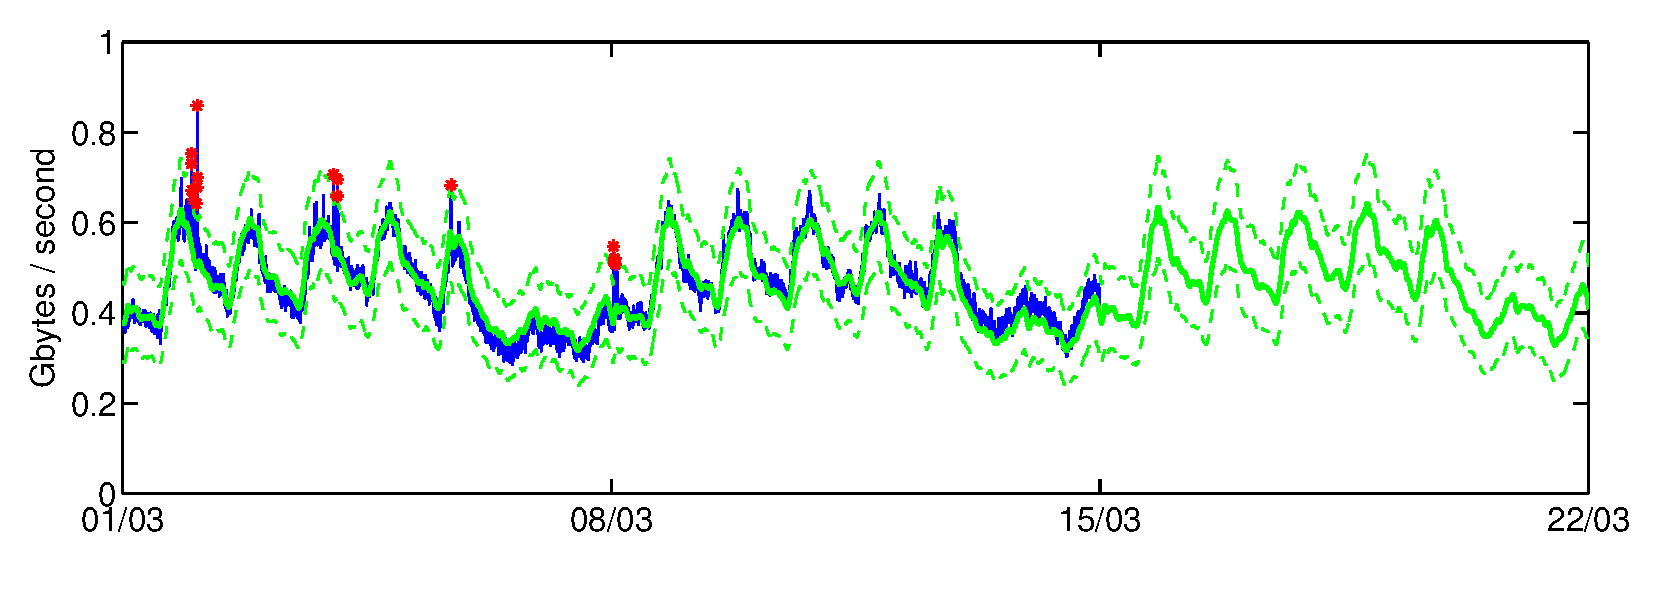
\includegraphics[width=\oneup]{Abilene_2004_decomp_1.eps}
    \caption{Results of decomposing traffic into components. The blue
      curve shows the original Abilene traffic from
      \autoref{fig:abilene_2004_b} (note that the data is missing for
      the third week). The solid green line shows $\hat{m}(t)=
      \hat{S}(t)\, \hat{L}(t)$, the estimated  mean, and the dashed
      green lines show the bounds of normal variation around this
      mean. The red asterisks indicate the anomalies $I(t)$.
      \label{fig:decomposition}}
  \end{center}
\end{figure}

Another feature of this model is the preservation of the properties of the
model through a linear combination, advantageous when looking at the
aggregated behaviour of the OD flows. Consider $K$ aggregated OD
flows, then 
\[
  x_{\text{agg}}(t) = \sum_{i=1}^K m_i(t) + \sum_{i=1}^K \sqrt{a_i m_i(t)} W_i(t) + \sum_{i=1}^K I_i(t). 
\]

\noindent The mean of $x_{\text{agg}}(t)$ is simply $m_{\text{agg}}(t)
= \sum_{i=1}^K m_i(t)$, and the peakedness is the weighted average of
the component peakedness, $a_{\text{agg}} =
\tfrac{1}{m_{\text{agg}}(t)} \sum_{i=1}^K a_i m_i(t)$. The linearity
properties allow $x_{\text{agg}}(t)$ to be expressed in the same form
as \autoref{eq:temporal_model} with the new parameters
$m_{\text{agg}}(t)$ and $a_{\text{agg}}$. The linearity property
enables the consistent computation of the variances of the aggregated
traffic, which is useful for network planning and analysis. Besides
this, \cite{Roughan02BRvariable} demonstrated the ease of estimating
the parameters of model \autoref{eq:temporal_model}, via simple
estimators and filtering.

The cyclical nature of the aggregated OD flows is also amenable to
Fourier analysis. The Fourier transform decomposes a periodic signal
into a weighted sum of sinusoids with distinct frequencies and
phases. It would be reasonable to assume the observed cycles can be
represented by a small number of Fourier coefficients (this does not
require that the signal be exactly sinusoidal as any periodic signal
can be approximated by a limited number of sinusoids). Indeed, it has
been demonstrated this is the case with the traffic volumes
\cite{Soule04TMLargest,eriksson10:_basis}, where as little as just
5 Fourier coefficients were needed to achieve low error in fitting
large OD flows of a Tier 1 network, demonstrating the relatively few
significant frequencies present in a diurnal cycle of the OD
flows. 

\autoref{fig:fourier} shows a similar analysis of Abilene data from
\autoref{fig:abilene_2004_b}. It shows a simple example of the
excellent degree of approximation to traffic we can obtain using only
a very small number of Fourier coefficients corresponding to daily
periods. 
\begin{figure}[thbp] 
  \begin{center}
    \mbox{ }\hfill
    \begin{subfigure}[b]{\twoup}
      \centering
      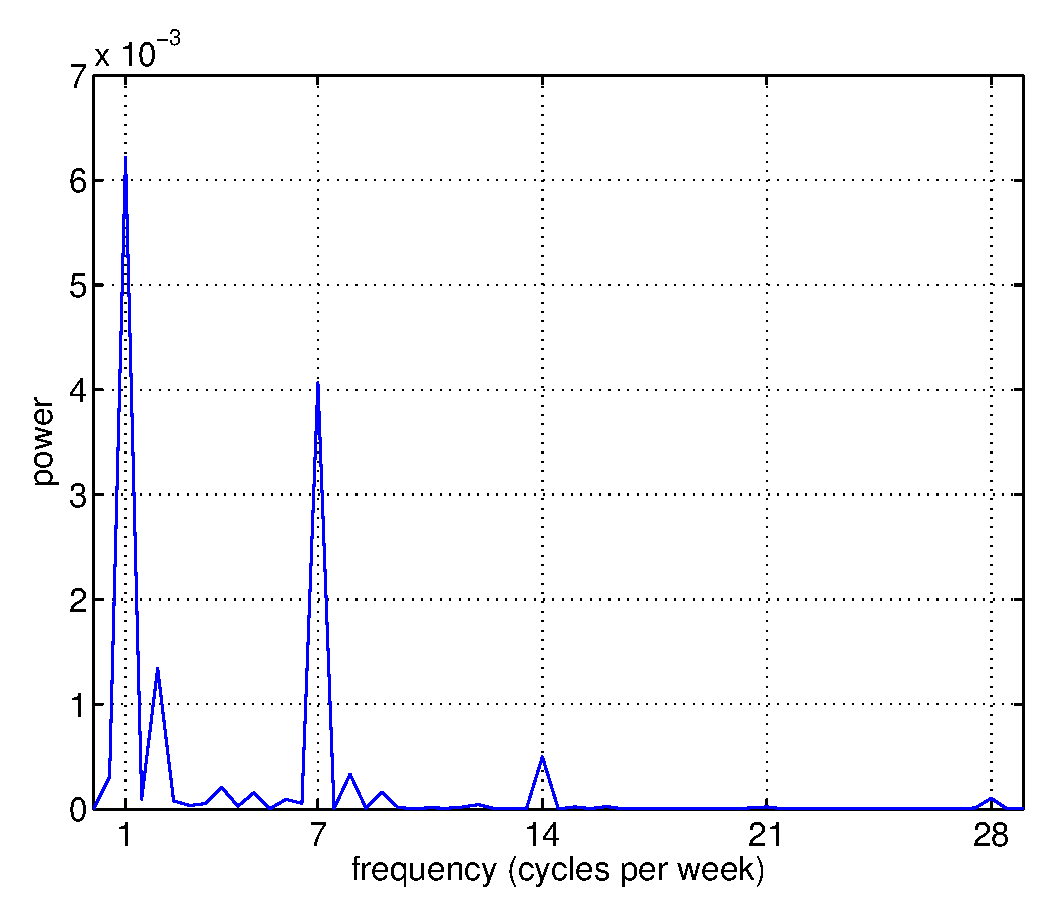
\includegraphics[width=\textwidth]{Abilene_2004_fourier_sprectra.eps}
      \vspace{-5mm}
      \caption{Fourier spectra (technically a periodogram) of the
        Abilene data.}
      \label{fig:fourier_a}
    \end{subfigure}
    \hfill
    \begin{subfigure}[b]{0.47\textwidth}
      \centering
      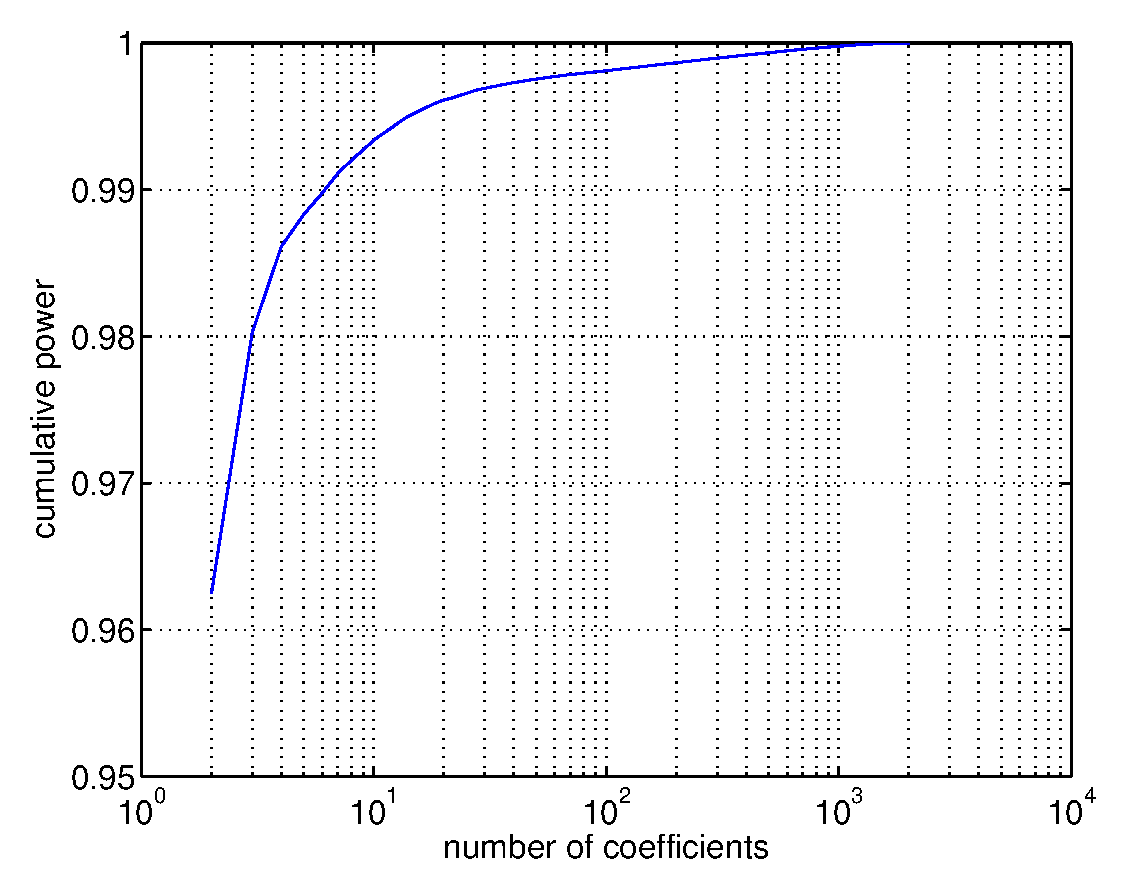
\includegraphics[width=\textwidth]{Abilene_2004_fourier_cum_power.eps}
      \vspace{-5mm}
      \caption{Cumulative power captured by Fourier components
        (sorted in descending order).}
      \label{fig:fourier_b}
    \end{subfigure}  
    \hfill \mbox{ }

      \vspace{5mm}
    \begin{subfigure}[b]{\oneup}
      \centering
      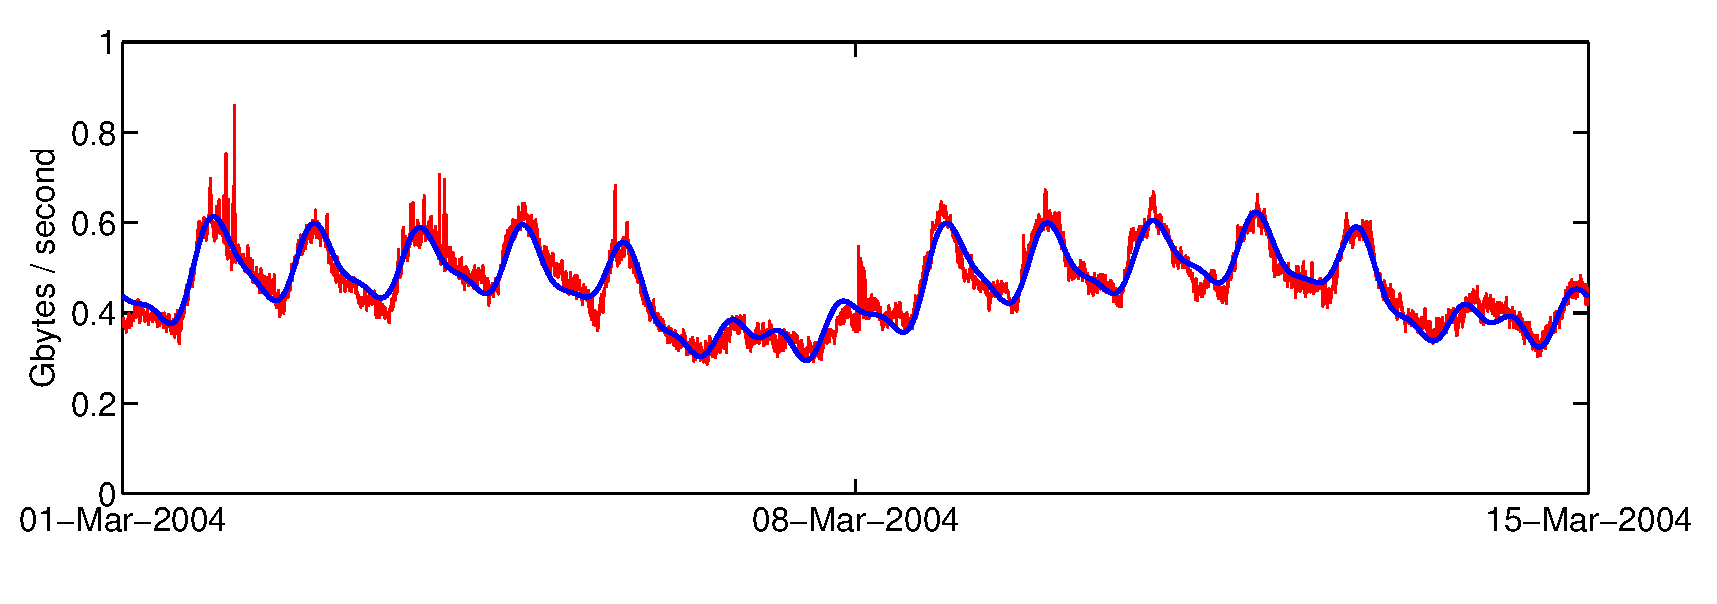
\includegraphics[width=\textwidth]{Abilene_2004_fourier_model_10.eps}
       \vspace{-9mm}
     \caption{Fourier approximation to the data using 10 (complex) coefficients.}
      \label{fig:fourier_c} 
    \end{subfigure}  

      \vspace{5mm}
    \begin{subfigure}[b]{\oneup}
      \centering
      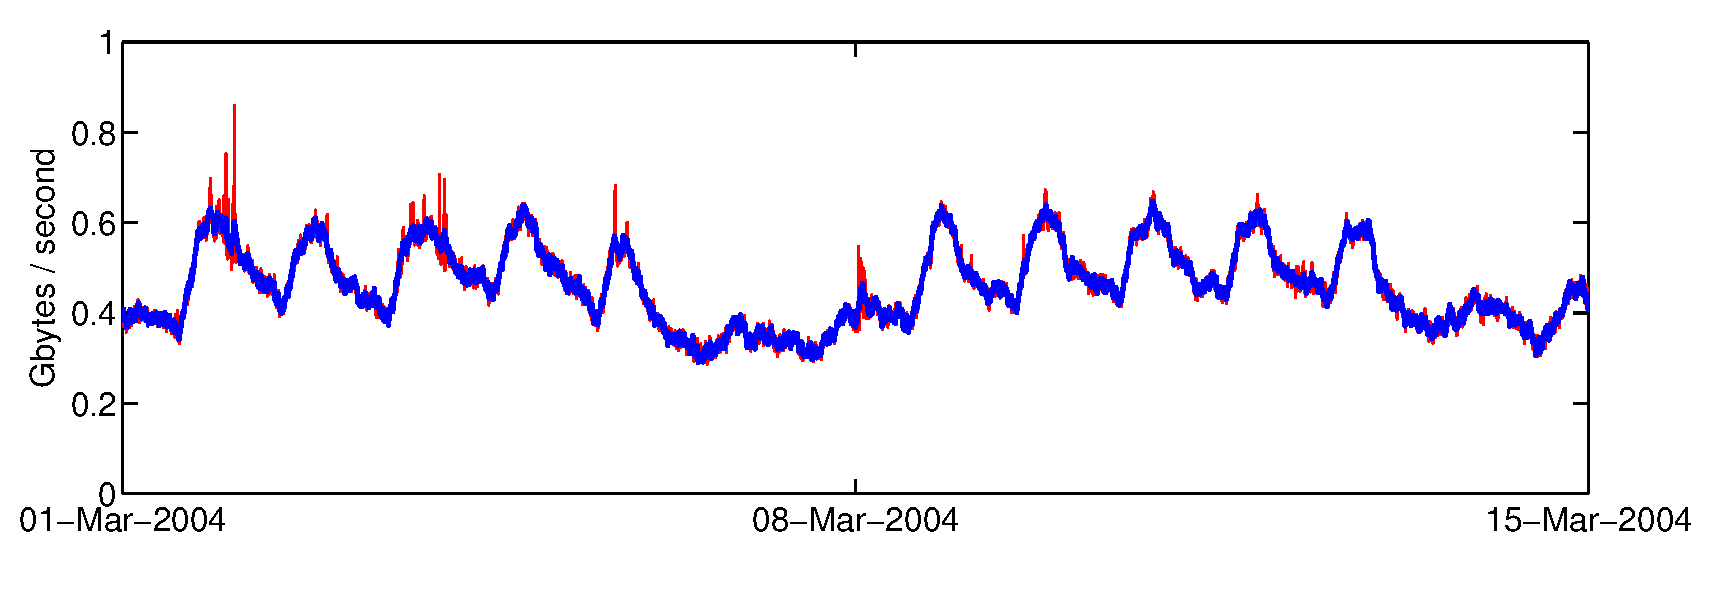
\includegraphics[width=\textwidth]{Abilene_2004_fourier_model_100.eps}
      \vspace{-9mm}
      \caption{Fourier approximation to the data using 100 (complex) coefficients.}
      \label{fig:fourier_d}
    \end{subfigure}  
   
    \caption{Fourier analysis of Abilene data shown in \autoref{fig:abilene_2004_b}. Blue curves represent the
    Fourier approximation of the traffic, indicated by the red curves.\label{fig:fourier}}
  \end{center}
\end{figure}         
\autoref{fig:fourier_a} shows the periodogram of the data
(the absolute magnitude of the Discrete Fourier Transform (DFT)). We
can see that only a few peaks (with frequencies of 1, 2, 7, and 14
cycles per week, corresponding to daily and weekly cycles and their
harmonics) are large enough to matter for gross features.
\autoref{fig:fourier_b} shows the cumulative power contained in the
largest of the Fourier coefficients, clearly showing that a small
number of these represent the power of the signal
well. \autoref{fig:fourier_c} shows an approximation of the original
signal using only 10 coefficients. We can see that the cyclic
components of the data are represented well, though the actual signal
varies around that noisily. Including additional components provides a
better approximation (in the sense of fitting the data more
accurately), but we can see that we are simply recreating the
noise. There is a clear tradeoff here between noise and signal, with
no absolute standard for the correct choice, but the underlying
promise of Fourier analysis is obvious.

The choice of time interval to use in Fourier analysis/approximation
is interesting. A longer interval provides more data, and hence better
estimates if the data is truly {\em cyclostationary}\footnote{A
  cyclostationary process can be thought of as one whose component
  processes formed from times embedded at multiples of the fundamental
  period from stationary sequences.}. However, as we discussed earlier, 
  there are noticeable
% http://en.wikipedia.org/wiki/Cyclostationary_process
trends in the overall volume, and so it is reasonable to assume that
there will sometimes be significant shifts in the pattern (with
respect to time of day or time of week). In these cases, extending the
length of the dataset can confuse the statistical variability with
non-stationary effects, resulting in biased estimates. The best
tradeoff appears to depend on the dataset, but periods of perhaps a
month seem to work reasonably well for estimating weekly cycles. 

However, there are alternative tools for such analysis, designed to
provide some flexibility in the tradeoff between time and
frequency. The simplest is perhaps the Short-Time Fourier Transform,
in which the signal is {\em windowed}, and the standard DFT is applied
to the windows of data to produce a {\em spectrogram}. The technique
has been applied in \autoref{fig:spectrogam} to a longer (6
weeks) sequence of the Abilene data. This segment of the data is more
challenging, as it contains many anomalies, \eg~the frequent spikes
in the traffic, or the drop in traffic on the Independence Day holiday,
observed on July 5th in 2004\footnote{Independence Day is actually 
celebrated on July 4th, but in 2004, the day falls on a Sunday. Thus, the following
day was declared a public holiday as well.}. \autoref{fig:spectrogam_a} shows the
set of data under consideration, along with its approximation using 10
coefficients. \autoref{fig:spectrogam_b} shows a spectrogram with
windows of length 1 week, and here we can still clearly see the weekly
and daily cycles appearing in most of the
windows. \autoref{fig:spectrogam_c} shows a spectrogram using 1 day
windows, with overlapping windows to smooth the results. The resulting
picture is poor at showing the cyclical behaviour of the traffic, but
clearly highlights the large anomalous spikes in the traffic in second
week of the data. 

\begin{figure}[thbp] 
  \begin{center}
    \begin{subfigure}[b]{\oneup}
      \centering
      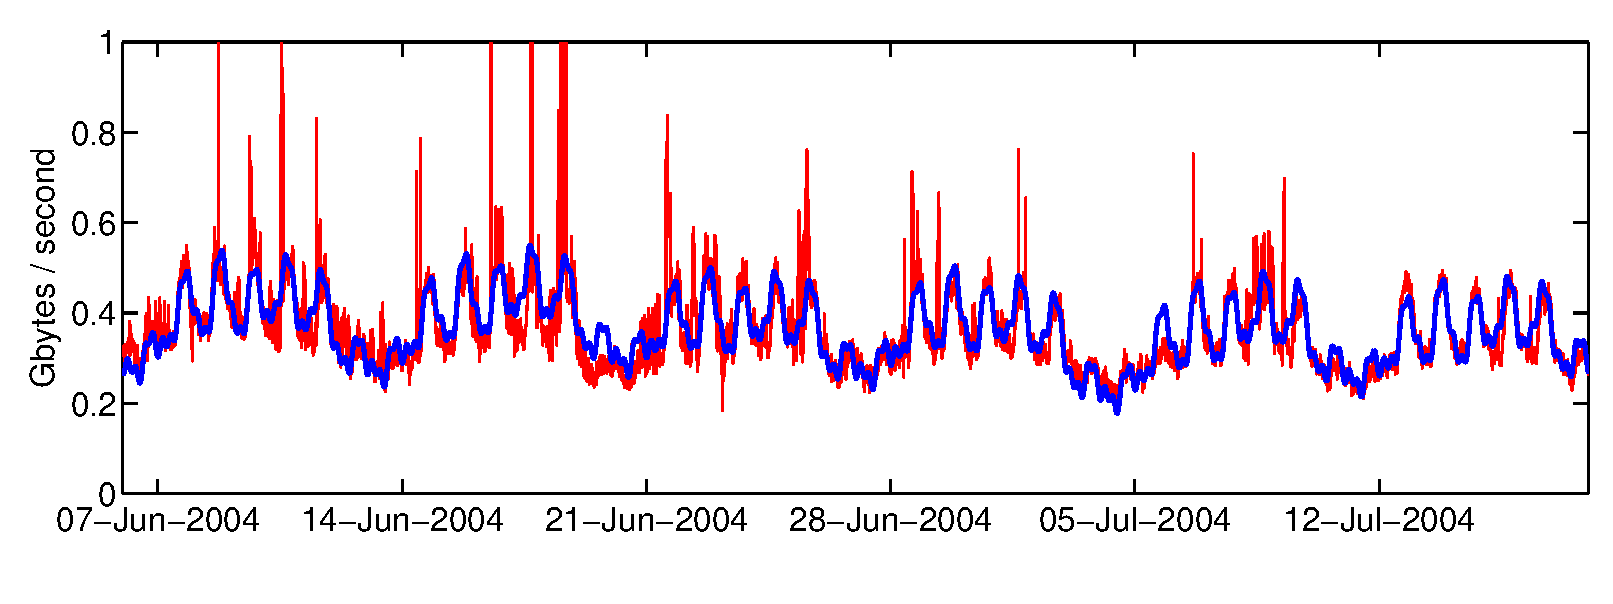
\includegraphics[width=\textwidth]{Abilene_2004_spectrogram_input.eps}
       \vspace{-9mm}
     \caption{Six weeks of Abilene data.}
      \label{fig:spectrogam_a} 
    \end{subfigure}  

      \vspace{5mm}
    \begin{subfigure}[b]{\oneup}
      \centering
      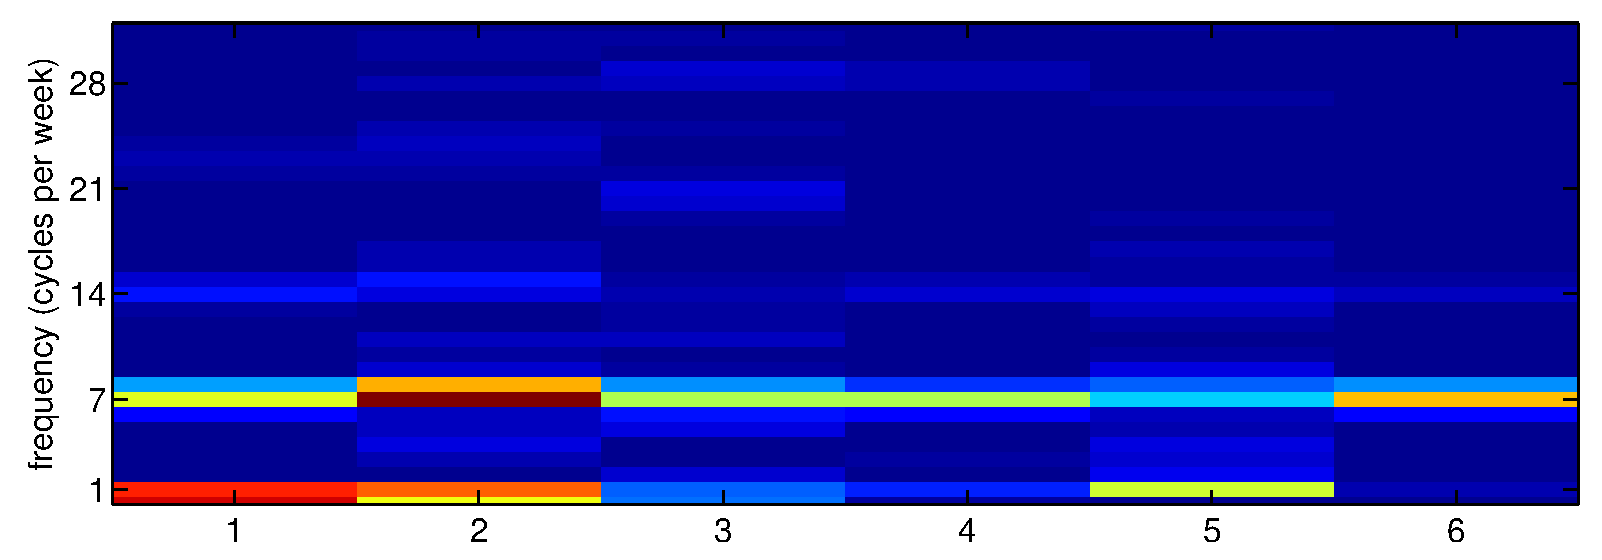
\includegraphics[width=\textwidth]{Abilene_2004_fourier_spectrogram_week.eps}
       \vspace{-5mm}
       \caption{Spectrogram with weekly windows. Brighter colours
         indicate more power. Again we see strong power at 1 and 7
         cycles per week, though the strength of these varies per
         week. For instance, in week 5 (when the Independence Day
         holiday was held) there was a week day, whose traffic more
         closely resembled weekend traffic, breaking the weekly cycle,
         and pushing more power into the daily cycle.}
      \label{fig:spectrogam_b} 
    \end{subfigure}  

      \vspace{5mm}
    \begin{subfigure}[b]{\oneup}
      \centering
      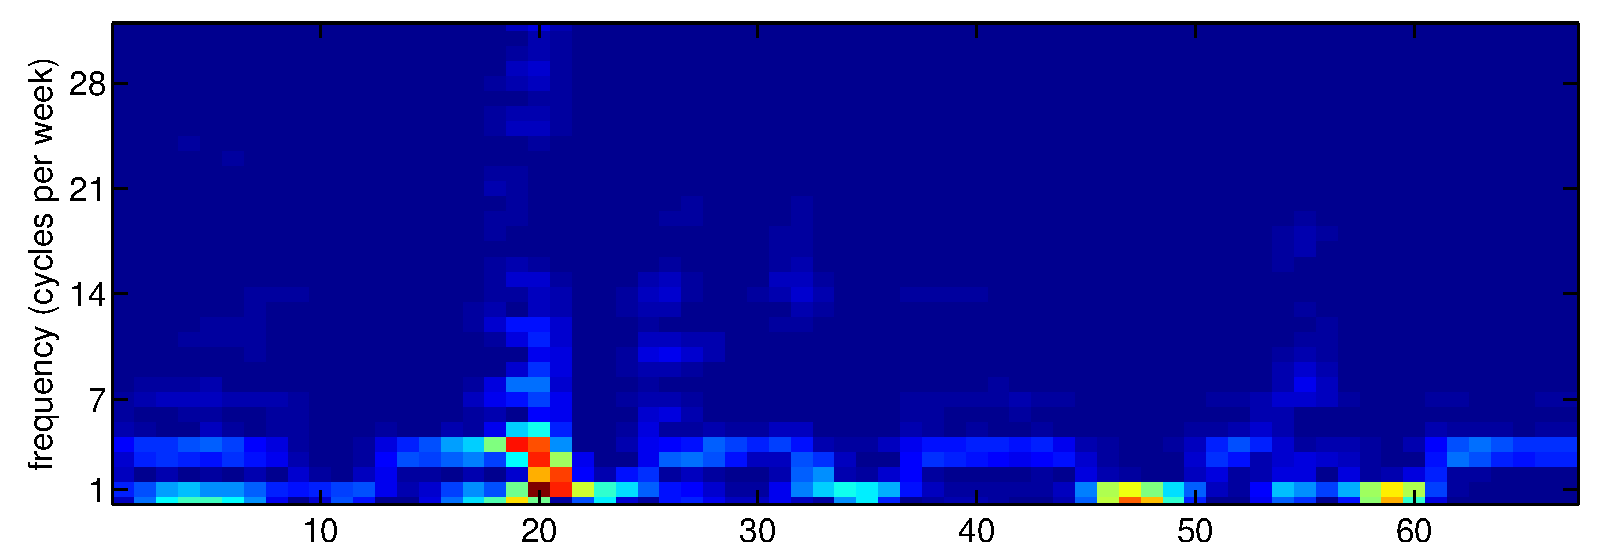
\includegraphics[width=\textwidth]{Abilene_2004_fourier_spectrogram_day.eps}
      \vspace{-5mm}
      \caption{Spectrogram with daily windows. Note that the
        time-resolution in this case is actually poorer than the image
      would suggest, accounting for the poor resolution of the daily
      and weekly cycles in this figure. However, the large anomalous
      spikes of traffic in the second week stand out clearly in this
      view, as they spread power across a range of frequencies.}
      \label{fig:spectrogam_c}
    \end{subfigure}  
   
    \caption{Short-Time Fourier analysis of Abilene data.\label{fig:spectrogam}}
  \end{center}
\end{figure}         

An even more powerful set of techniques that have been applied to the
temporal analysis of traffic are the Wavelet
transforms~\cite{Veitch97Wavelet,Barford02Anomaly,Papagiannaki05Long},
which provide a more flexible set of time/frequency
tradeoffs. Wavelets have also been applied to spatial analysis of
traffic matrices 
\cite{CrovellaKolaczyk03,CoatesCompressedNetworkMonitoring,wang10:_wavel_based_traff_matrix_model,rincon08:_dw,roughan_mra_09},
which we will consider in a moment.  However, wavelets are a
relatively complicated set of techniques, and it is outside the scope
of this chapter to provide an introduction to that material. See for
instance \cite{mallet:_book} for more information. 

Principal components analysis (PCA) has also been employed to quantify
the temporal correlations of the traffic matrix. If $\cX$ is a matrix
where the rows represent a measurement (for instance an OD flow) and
columns represented traffic volumes at time $t$, then temporal PCA
decomposes the matrix $\cX^\T \cX$ into its corresponding components
of eigenvalues and eigenvectors. Often, each column is \emph{centred}, simply by
subtracting the mean vector $\bar\bx$, the average of all columns, from each 
column in $\cX$. In what follows, $\cX$ is assumed to be centred.

The matrix $\cX^\T \cX$ is \emph{positive
semidefinite}. Visualising this geometrically, if the columns of the matrix is reinterpreted
as a set of points, then they trace out an ellipsoid. Alternatively, $\cX^\T \cX$
may be viewed as the \emph{empirical covariance matrix} of the columns of
$\cX$, in effect computing temporal correlations in traffic. 

PCA is used to find the directions of greatest variance of $\cX^\T \cX$
by decomposing $\cX^\T\cX = \bW \bD \bW^\T$, where $\bW$ is an orthonormal matrix 
containing the eigenvectors of $\cX^\T\cX$ and $\bD$ the diagonal 
matrix containing the eigenvalues of $\cX^\T\cX$. The eigenvectors
are known collectively as the \emph{principal axes}. The eigenvectors are ordered in a 
non-decreasing order with respect to their associated eigenvalues, starting from the
eigenvector associated with the largest eigenvalue to the smallest. An equivalent view
is that PCA essentially performs a Singular Value Decomposition (SVD) of the matrix
$\cX$, by computing only its right singular basis $\bW$.

Thus, every row of $\cX$ can be expressed as $\bx_k =  \baa^\T_k \bW^\T$, 
\ie~a linear combination of a coefficient vector
$\baa_k$, called the \emph{principal components}. Here, $\bW$ is equivalent to a linear
transform, post-multiplied to the data. Intuitively, if the size of the set of
principal axes with large principal components are small, then this is evidence
there are high temporal correlations between the traffic flows. In practice, it is
common to focus on the few largest principal axes for the purpose of data reduction.
Basically, this means choosing the first few significant columns of $\bW$ to approximate each
$\bx_k$ with $\tilde\bx_k$ such that $\|\bx_k - \tilde \bx_k\|_2 < \epsilon$, for some 
small error $\epsilon > 0$.

As an aside, PCA may be performed on $\cX\cX^\T$, in effect computing the spatial
correlations of $\cX$ instead. Here, we have $\cX\cX^\T = \bV \tilde\bD \bV^\T$, with
each column $\bar\bx_k = \bV \tilde \baa_k$, equivalent to $\bV$ pre-multiplied
with the data. Spatial PCA was used in the context of anomaly detection
\cite{Lakhina04Anomaly,Lakhina04Diagnosing,Lakhina05Mining} but there are problems
with this approach. These discussions are deferred to \autoref{sec:applications}.

\begin{figure}[thbp] 
  \begin{center}
     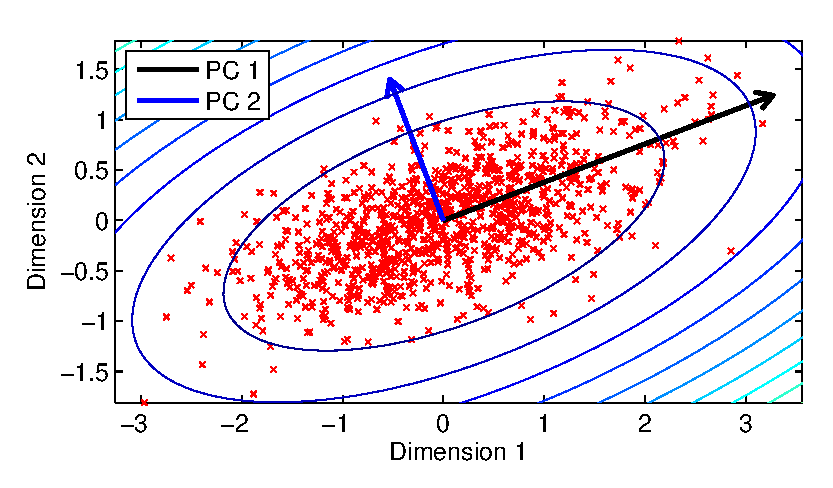
\includegraphics[width=0.7\textwidth]{PCA_example.eps}
    \caption{Principal components analysis of the empirical covariance matrix of a two dimensional 
    data matrix of 1000 centred points $\cX$. Here, ``PC 1''  and ``PC 2'' are the principal 
    components. Note the elliptical shape of the contours of the
    density with semi-major and semi-minor axis given by the first and
    second principal components, respectively.  \label{fig:pca}}
  \end{center}
 \end{figure}
 
\autoref{fig:pca} demonstrates an example of PCA performed on the covariance matrix of 
1000 two dimensional data points with zero mean, \ie~$\cX$ has 2 rows and 1000 columns. 
The matrix $\cX^\T \cX$ formed by the data points vaguely resembles an ellipse. Here, there
are two principal components, denoted by  ``PC 1''  and ``PC 2'', with the higher variance
captured by PC 1. This is clear from the way the points on the figure
are distributed. The key point to take away is that both components capture the direction
of highest variance and are orthogonal to each other.  Moreover, the principal components matrix 
$\bW$ has PC 1 and PC 2 as its first and second columns respectively. Each data point 
can be expressed as linear combination of these two components. The concept is easily
extended beyond two dimensions to the larger dimensions typically encountered with
traffic matrices.

PCA was performed by Lakhina \etal on empirical data from two backbone networks show
that OD flows are a combination of no more than 35 ``eigenflows'' (the principal axes), and
in fact, fewer than this in general \cite{Lakhina04TrafficStruct}, out of over 100 OD flows. 
These eigenflows belonged to one of three categories, depending on their properties:
\begin{enumerate}
\item \textbf{deterministic or $d$-eigenflow}: generally the
  significant diurnal component of the largest OD flows. Although
  present in smaller OD flows, these eigenflows are less
  significant. These eigenflows have a cyclo-stationary property and
  suggests that these eigenflows may be approximated by a small number
  of Fourier coefficients. These eigenflows account for the majority
  of the total traffic of the OD flow.
\item \textbf{spike or $s$-eigenflow}: medium sized eigenflows with a
  spikiness behaviour in time, with values ranging up to 5 standard
  deviations from the mean of the OD flow. This suggests these
  contributions come from bursty processes and may be modelled by a
  wideband Fourier process.
\item \textbf{noise or $n$-eigenflow}: small eigenflows behaving like
  stationary additive white Gaussian noise. These eigenflows have
  small energy and their contribution to overall traffic is
  negligible. The majority of eigenflows from Lakhina {\em et al.}'s datasets
  belong to this category.
\end{enumerate}
There are several eigenflows belonging to two or more categories, but
these eigenflows are rare \cite{Lakhina04TrafficStruct}.  For the most
part, these categories are very distinct for almost all
eigenflows. The low number of eigenflows compared to the dimension of
the traffic matrices under study suggests low intrinsic dimensionality
of traffic matrices, although the upper bound of 35 eigenflows indicates that the OD traffic
is only ``approximately'' low rank. The results show a power law-type distribution
of the principal components \cite{Lakhina04TrafficStruct}. The decay of the
distribution varies depending on the ISP, with some distributions
exhibiting a very fast decay and some much slower decay.

In many senses PCA confirms the previous analysis
and modelling, but it is interesting because its approach simply looks
for correlations across different sets of measurements, and uses a
different set of assumptions from, for instance, Fourier analysis
which can be performed on a single time series.

Finally, it is important to note that the full data needs to be
available (no missing entries in $\cX$) in order to perform
PCA. Furthermore, the basic flavour of PCA as described above is not a
robust method, since it is an entirely data driven method and is
therefore sensitive to outliers~\cite{Ringberg07PCA}. Robust variants
have been proposed but they necessarily complicate the basic version
of PCA presented here, since these modifications entail constructing
methods to identify and exclude outliers. Despite these disadvantages,
in its purest form, PCA is a useful tool to learn the temporal
structure of traffic flows.

\subsection{Spatial Modelling}

Spatial models only focus on the properties of traffic between source
and destination pairs, typically within a single measurement interval,
without regard to how the traffic changes in time. The models
presented here are the gravity model and its generalisations, the
discrete choices model, the independent connections model and low rank
spatial model. However, we shall start with the simplest test models. For ease of
exposition in this section, the set of sources and destinations are
assumed to be sets of PoP ingress and egress nodes, denoted by $\cI$
and $\cE$ respectively. The set $\Omega$ represents the set of all
nodes in the network, \ie~$\Omega = \cI \cup \cE$.

\subsubsection{Simple {\em test} models}

We must remember that the purpose of models is not always to
``realistically'' represent a network's traffic. Their purpose is to
provide inputs to other tasks. One common task is to assess the
sensitivity of a network to different types of traffic, and to that
end, engineers can consider the effect of various artificial {\em test}
models. 

Three such are the uniform traffic model, peak load model, and
focussed overload model. They are extremely simple:
\begin{description}
\item[uniform] this simple model assigns the same value to all
  traffic matrix elements. It is used to provide a base load in some
  experiments, or to see the behaviour of a network under one extreme
  (the most uniform extreme) of traffic \cite[Chapter 4.5.1]{Cahn98WANDesign}.

\item[peak load] this model is equally simple, and equally extreme. It
  has zero for all loads except one OD flow. It simulates the opposite
  extreme where the aim is to see the effect of one dominant flow.

\item[focussed overload] this type of traffic matrix simulates the effect of a
  {\em focussed overload}, or {\em flash crowd}\footnote{See also the
    slashdot effect.}, where many users become interested in one
  location or resource and the traffic to this single location from
  all other sources is the dominant effect in the network. As a
  result, the focussed overload can be represented by a matrix with all
  elements zero, except for one row. We can likewise represent a
  focussed traffic load arising from a single point (say as response
  traffic to a focussed set of queries) by a matrix with a single
  non-zero column.
\end{description}
The advantage of each of the models lies in its simplicity. The
simplicity means that the effect of the traffic is easy to interpret,
and thus gain insights from these models where a more complex
model would perhaps confound us with multiple potential causes for
some results. For instance, in each of the above models we can
gradually increase the traffic to see when capacity bounds are
reached, and where those bounds would be reached in order to identify
potential bottlenecks in a network.

Other test models based on classical distributions such as the Poisson
and Gaussian distributions were proposed by Vardi \cite{Vardi96Tomo},
and Tebaldi and West \cite{Tebaldi98Tomo} and Cao \etal 
\cite{Cao00Tomo}, respectively. Their well-known properties make it easy
to analyse results and provide insights, at the cost of a departure from 
real traffic properties.

\subsubsection{Gravity model}

The gravity model is perhaps the next simplest type of model, but it
has a great deal to offer. Here, traffic from the source to the destination
are modelled as a random process. In its simplest form it assumes, any
packet originating a source to a destination nodes are \emph{independent}
of other packets. 
Depending on context, this could be the origin and destination, or ingress
and egress nodes respectively.  Consequently, the traffic between 
two nodes is \emph{proportional} to
the total traffic from the source node to the destination node. The
gravity model is amongst one of the most well-studied
models and is considered a canonical first generation model.

The name of the model derives from Newton's model of gravitation,
where the gravitational force is proportional to the product of the
mass of two objects divided by the distance between them squared. The
general formulation of the gravity model is defined by two forces: the
\emph{repulsive} force (factor) $R_i$, associated with ``leaving''
from $i$ and the \emph{attractive} force (factor) $A_j$, associated
with ``going'' into $j$. Its general form is described by the
following equation: \be X_{i,j} = \frac{R_i \,A_j}{f_{i,j}},
\label{eq:grav_model}
\ee where $f_{i,j}$ represents the \emph{friction factor}, which
describes the weakening of the forces (akin to distance in Newton's
model), depending on the physical structure of the modelled
phenomenon. The model has been used extensively in various fields, for
instance the modelling of street traffic~\cite{potts72}. 
 
In the context of Internet traffic matrix modelling, the friction
factors have typically been taken to be constant. That is, distance is
assumed to have little effect on network traffic. That certainly
seemed to be true even at a fairly large scale in the past, but it is
unknown to what extent the deployment of CDNs (Content Distribution
Networks) over the last few years has changed distance dependence, 
since CDNs locate traffic closer to the end user to avoid paying for
transit costs across the network, or
how inter-country matrices are affected by distance (for instance
through language barriers). Where distance is ignored, equation
\autoref{eq:grav_model} becomes 
\be X_{i,j} =
\frac{X_i^{\text{in}}\, X_j^{\text{out}}}{X^{\text{total}}},
\label{eq:network_grav}
\ee
where $X_i^{\text{in}}$ is the total traffic entering the
network through $i$, $X_j^{\text{out}}$ is the total traffic exiting
the network through $j$ and $X^{\text{total}}$ is the total traffic
across the network \cite{Zhang03Fast}. The model can be expressed
succinctly as the single rank matrix 
\be 
\bX =
\frac{\bx^{\text{in}}\, \left.\bx^{\text{out}}\right.^\T}{X^{\text{total}}}.
\label{eq:network_grav_mtx}
\ee
The popularity of the model stems from the ease of
estimating the $X_i^{\text{in}}$ and $X_j^{\text{out}}$ for each node
pair $(i,j)$, and especially at the PoP or backbone level, since the
level of traffic aggregation mitigates errors in the estimation of
these quantities from sampled traffic.

The gravity model only captures the spatial structure of the
traffic. The key assumption of the gravity model is the independence
between each source $i$ and destination $j$. Coupled with the
assumption that none of the nodes act as a source or sink of traffic
(\ie~that traffic is conserved in the network) $X^{\text{total}} =
\sum_{k \in \cI} X_k^{\text{in}} = \sum_{\ell \in \cE}
X_\ell^{\text{out}}$. Under normal operating conditions in most
backbone routers, where congestion is kept to a minimum, the
conservation assumption appears reasonable. With this assumption,
\be
X_{i,j} = X^{\text{total}}\, p_i^{\text{in}}\, p_j^{\text{out}},
\label{eq:network_grav_normalised}
\ee
where
\ben
p_i^{\text{in}} 
    = \frac{X_i^{\text{in}}}{\sum_{k \in \cI} X_k^{\text{in}} },
\quad \mbox{ and } \quad 
p_j^{\text{out}} 
    = \frac{X_j^{\text{out}}}{\sum_{\ell \in \cE} X_\ell^{\text{out}}},
\een
are the proportions of traffic entering the ingress and
exiting the egress nodes respectively, called \textit{fanouts}. The
formulation \autoref{eq:network_grav_normalised} is known as the
\emph{fanout} formulation because it describes how a packet entering
via node $i$ is distributed to several nodes $j \in \cE$. Fanout has
been demonstrated to be close to a constant over several measurement
intervals, compared to the traffic matrix \cite{Medina02TMdirections},
suggesting the fanout may be a better alternative to measure and use
in, for instance, anomaly detection, than the raw traffic volumes.

Observe the implication of independence between the source and
destination in \autoref{eq:network_grav_normalised}: $\Pr(\cI,\cE) =
p_\cI^{\text{in}} p_\cE^{\text{out}}$. An immediate consequence is
$\Pr(\cE\,|\,\cI) = P_d(\cE)$, where $P_d(\cE)$ is the marginal
distribution of the traffic demand distribution at the
destinations. The assumption of independence between the source and
destination leads to two important properties of the gravity model
making it well suited to traffic matrix modelling.

\begin{thm}[Independence]
  Independence between the source and destination traffic holds for
  any randomly chosen submatrix of the model.
  \label{thm:independence}
\end{thm}
\begin{proof}
  The independence property implies $\Pr(s,d) = p_s^{\text{in}}\,
  p_d^{\text{out}}$, holding for every $s \in \cI$ and $d \in \cE$.
  This condition would also hold for a subsample of locations in $\cI$
  and $\cE$.
\end{proof}

\begin{thm}[Aggregation]
An aggregate of the gravity model is itself also a gravity model. 
\label{thm:aggregation}
\end{thm}
\begin{proof}
  Let all nodes be partitioned into $N$ subsets $\{\cS_1,\cS_2,
  \cdots,\cS_N\}$, with $\cS_i \cap \cS_j = \emptyset$ for $i \ne j$
  and $\cup_{i=1}^N \cS_i = \Omega$. The aggregated traffic matrix is
  defined as \be X_{\cS_i,\cS_j} = \sum_{i \in \cS_i} \sum_{j \in
    \cS_j} X_{i,j}.
\label{eq:aggregated}
\ee
The independence condition implies 
\be
X_{i,j} = \frac{X_{i,\Omega} \, X_{\Omega,j}}{X^{\text{total}}}.
\label{eq:independence_model}
\ee
Substituting \autoref{eq:independence_model} into \autoref{eq:aggregated}, 
\begin{align*}
X_{\cS_i,\cS_j} &= \sum_{i \in \cS_i} \sum_{j \in \cS_j} \frac{X_{i,\Omega} \,X_{\Omega,j}}{X^{\text{total}}}
= \frac{1}{X^{\text{total}}} \sum_{i \in \cS_i} X_{i,\Omega} \sum_{j \in \cS_j} X_{\Omega,j}\\
&=  \frac{X_{\cS_i,\Omega} \, X_{\Omega,\cS_j}}{X^{\text{total}}}.
\end{align*}
which is also a gravity model.
\end{proof}

These are not just theoretical results. Any model should be consistent
in the sense that if the data to which it applies is viewed in a
different way (for instance by sampling or aggregation) then the model
should still apply (though its parameter values may change). It seems
like an obvious requirement, and yet there are many models to which it
does not apply. 

The utility of the gravity model is not just restricted to network
measurement. It is used in various areas: teletraffic modelling
\cite{Kowalski95TeleModel,Lam97Teletraffic}, economy and trade
\cite{Pyhnen63Trade,Tinbergen62Econ}, epidemiology
\cite{Ferrari06Pollinator,Murray77Measles,Xia04Measles}, sociology
\cite{Stewart48Socio}, the retail industry, specifically Reilly's law
of retail gravitation
\cite{Converse49RetGravNew,Jung59RetailGravTrue,Reynolds53RetailGrav},
and in vehicular traffic modelling \cite{Erlander90GravTransport}. More
advanced discussion on the gravity model (albeit with an economics
flavour) is found in \cite{Sen95Gravity}.

The gravity model can be interpreted in terms of the \emph{principle
of maximum entropy}. Entropy here is the Shannon entropy from
information theory parlance \cite{Cover06InfoTheory}. The principle is
closely related to Occam's Razor, essentially choosing the
parsimonious explanation of the data amongst competing
explanations. With little information regarding the traffic matrix
besides the total traffic information, it turns out that the best one
can do, according to the principle, is to describe the observations
with a model promoting independence and symmetry, consistent with
known constraints.  In this way, the model enjoys robustness compared
to other models, as the gravity model seeks to minimise deviation from
what has already been observed.

The model, however, is not without its drawbacks. The main critique
against the gravity model is in its main assumption: the independence
of the ingress and egress nodes\footnote{The difference between OD and
  IE traffic matrices becomes critical here.}. It has been pointed out
in several papers \cite{Erramilli06IndepConn} that this assumption
does not hold true. Most traffic between node pairs are determined by
connections, for example TCP initiated sessions, so there exist
dependencies between node pairs. The second is the violation of the
conservation of traffic assumption, for \eg~when there is high
congestion, causing packets to be dropped from router queues.

Actual traffic matrices are generally asymmetric, violating the main assumption
of gravity models. For example, forward traffic volumes of a source-destination
pair of nodes do not typically match up with the volume of reverse
traffic.  Even if the OD traffic matrix matches the gravity model
well, the corresponding IE traffic matrix may be vastly different, due to hot
potato routing \cite{Teixeira04PotatoSIG}.

Hot potato routing is implemented as a part of the BGP 
decision process \cite{Rekhter1995BGP}. BGP allows 
network operators to choose the egress points of traffic at the 
prefix level. The decision may also vary across a network so 
that traffic at different points  can end up being routed to 
different egress points. The idea of hot potato routing comes 
from its namesake: traffic is the ``hot
potato'' in this case and the network tries to get rid of the ``hot
potato'' as quickly as possible to avoid costs of transiting it over 
long distances. Therefore, traffic is sent on the shortest external 
route connecting an ingress to egress point. BGP provides less
control over ingress points and this is what leads to the 
fundamental asymmetry in the IE traffic matrix. 

An example of hot potato routing is in \autoref{fig:hot_potato}.
Here, there is a clear asymmetry since the paths taken by traffic flows from
Perth to Sydney differ from Sydney to Perth. 
To further understand hot potato routing, we refer the reader to 
 \cite{Caesar05BGP} for a basic understanding
of BGP routing policy.

\begin{figure}
  \hfill \HotPotatoIn \hfill \HotPotatoOut \hfill \mbox{ } \\
  \caption{Traffic flow between two ASes, one in Perth and the other in
    Sydney. Note the asymmetry in traffic: due to the action of hot
    potato routing, the path taken by a traffic flow from Perth to
    Sydney differs from the reverse path, since by BGP's implementation, 
    the closest external link of an AS is always chosen to route traffic out from the AS.}
  \label{fig:hot_potato}
\end{figure}

Thus, although the source-destination independence assumption may hold
for OD traffic matrices, it may not necessarily hold for IE traffic
matrices, due to distortion by inter-domain routing. Consider a simple
toy example of a network in \autoref{fig:gravity_example} (originally
from \cite{Alderson06Topology}). The ASes A, B and C are assumed to be
connected, with A having three routers: 1, 2 and 3. The inter-domain
routing protocol between these ASes uses hot potato routing, seeking
the shortest path between these ASes.

Suppose $X^{\text{total}} = 9$. Consider an OD traffic matrix with the form of a gravity model, with even spread of traffic over each 
internal router 1, 2 and 3, with $\bx^{\text{in}} = \bx^{\text{out}} = \bx$. The OD traffic matrix has the form $\bX_{\text{OD}} = \bx \bx^
\T/X^{\text{total}}$, with $\bx = (1,1,1,3,3)^\T$, and written explicitly as
\be
\bX_{\text{OD}}  = 
\begin{array}{lll}
       & \;\;1 \;\;\;\;\;\;\;  2 \;\;\;\;\;\;\; 3 \;\;\;\;\;\;\; \text{B} \;\;\;\;\;\;\; \text{C} \\
          \begin{array}{lll}
            1 \\
            2 \\
            3 \\
            \text{B} \\
            \text{C} \\
          \end{array} 
       & 
       \hspace{-4mm}
          \left( 
          \begin{array}{lllll}
         1/9 & 1/9 & 1/9 & 1/3 & 1/3 \\
         1/9 & 1/9 & 1/9 & 1/3 & 1/3 \\
         1/9 & 1/9 & 1/9 & 1/3 & 1/3 \\
         1/3 & 1/3 & 1/3 & 1   & 1   \\
         1/3 & 1/3 & 1/3 & 1   & 1   \\
          \end{array} 
          \right)
      \end{array}.
\ee
By \autoref{thm:aggregation}, the gravity model for the aggregated OD matrix, comprising OD traffic volumes between ASes A, 
B and C, is given by
\be
\bX'_{\text{OD}} =
 \begin{array}{lll}
       &   \text{A} \;\;\; \text{B} \;\;\; \text{C} \\
          \begin{array}{lll}
            \text{A} \\
            \text{B} \\
            \text{C} \\
          \end{array}
       &
       \hspace{-4mm}
          \left(
          \begin{array}{lll}
            1 & 1 & 1 \\
            1 & 1 & 1 \\
            1 & 1 & 1 \\
          \end{array}
          \right)
      \end{array}
\label{eq:OD_aggregate},
\ee
simply by summing the traffic in the internal nodes. In this case, $\bX'_{\text{OD}}  = \bx\bx^\T/X^{\text{total}}$, 
with $\bx = (3,3,3)^\T$, still a gravity model.

\begin{figure}[p]
\GravityEx
\caption{Example toy network with three ASes: A, B and C are all assumed to be peers. The routers 1, 2 and 3 are internal to A.}
\label{fig:gravity_example}
\end{figure}

\begin{figure}[p] 
  \begin{center}
    \begin{subfigure}[b]{\twoup}
      \centering
      \GravityInternal 
      \caption{Internal traffic within A.}
      \label{fig:traffic_routing_a}
    \end{subfigure}
    \hfill
    \begin{subfigure}[b]{\twoup}
      \centering
      \GravityIn
      \caption{Incoming traffic to A.}
      \label{fig:traffic_routing_b}
    \end{subfigure}  
    
    \begin{subfigure}[b]{\twoup}
      \centering 
      \GravityOut
      \caption{Outgoing traffic from A.} 
      \label{fig:traffic_routing_c}
    \end{subfigure}
    \hfill
    \begin{subfigure}[b]{\twoup}
      \centering
      \GravityExternal
      \caption{Traffic external to A.}
      \label{fig:traffic_routing_d}
    \end{subfigure}  

    \caption{Traffic flows within the network of
      \autoref{fig:gravity_example}, classified into four
      components.\label{fig:traffic_routing}}
  \end{center}
\end{figure}         


In order to construct the IE traffic matrix, the ingress and egress points of the network in A needs to be determined. The following
assumptions are made:
\begin{enumerate}
\item A, B and C are peers,
\item the shortest AS path protocol is used for inter-domain routing, 
\item hot potato routing is used internally by A, and
\item the Interior Gateway Protocol (IGP) weights are all equal.
\end{enumerate}
Suppose ingress and egress points are defined by the following routing table ($*$ represents a wildcard character)
 \begin{center}
\begin{tabular}{|c|c|c|}
\hline
  \textbf{Origin router} & \textbf{Destination}  & \textbf{Egress router} \\
  \hline
  1 & B & 2  \\
  1 & C & 3  \\
  2 & * & 2 \\
  3 & * & 3 \\
  \hline
\end{tabular}
\end{center}
The path for each traffic flow in the network, therefore, differs depending on its source 
and destination. 

All traffic flows between the PoPs may be decomposed into four components: internal traffic within A, traffic 
departing A, traffic coming into A and traffic external to A, shown in \autoref{fig:traffic_routing}. 
The internal traffic of A (\autoref{fig:traffic_routing_a}) is just the top-left $3 \times 3$ submatrix of $\bX_{\text{OD}}$, which is
\be
 \bX_{\rm internal} =  \begin{array}{lll}
       & \;\;\;  1 \;\;\;\;\;\;\;  2 \;\;\;\;\;\;\; 3  \\
          \begin{array}{lll}
            1 \\
            2 \\
            3 \\
          \end{array} 
       & 
       \hspace{-4mm}
          \left( 
          \begin{array}{lllll}
         1/9 & 1/9 & 1/9 \\
         1/9 & 1/9 & 1/9  \\
         1/9 & 1/9 & 1/9  \\
          \end{array} 
          \right)
      \end{array}
\ee
Traffic bound for A, as seen in \autoref{fig:traffic_routing_b} to be specifically for router 1 in this instance, from its peers has entry 
points controlled by B and C, given the above routing table. Hence, from A's point of view, the traffic behaves as if the traffic 
randomly distributed across ingress links. Assuming the traffic is evenly spread, the traffic matrix is 
\be
 \bX_{\rm arriving} =  \begin{array}{lll}
       & \;\;\; 1 \;\;\;\;\;\;\;  2 \;\;\;\;\;\;\; 3  \\
          \begin{array}{lll}
            1 \\
            2 \\
            3 \\
          \end{array} 
       & 
       \hspace{-4mm}
          \left( 
          \begin{array}{lllll}
         0 & 0 & 0  \\
         1/3 & 1/3 & 1/3  \\
         1/3 & 1/3 & 1/3  \\
          \end{array} 
          \right)
      \end{array}
\ee
Traffic departing from A, seen in \autoref{fig:traffic_routing_c} as originating from router 1, and routed by hot
potato routing, is described by
\be
\bX_{\rm departing} =  \begin{array}{lll}
       & \; 1 \;\;\;\;\;\;  2 \;\;\;\;\;\;\; 3  \\
          \begin{array}{lll}
            1 \\
            2 \\
            3 \\
          \end{array} 
       & 
       \hspace{-4mm}
          \left( 
          \begin{array}{lllll}
         0 & 1/3 & 1/3  \\
         0 & 2/3 & 0  \\
         0 & 0   & 2/3  \\
          \end{array} 
          \right)
      \end{array}
\ee
Since A does not provide transit for B and C, traffic external to A, \ie~between B and C, should not appear on A, the traffic will 
remain unseen by A (\autoref{fig:traffic_routing_d}). Thus, the total IE traffic matrix is the sum of the component traffic above, so 
that the entry and exit points match, and is given by
\be
\bX_{\text{IE}} =
 \begin{array}{lll}
          \left(
          \begin{array}{lll}
         1/9 & 4/9  & 4/9 \\
         4/9 & 10/9 & 4/9 \\
         4/9 & 4/9  & 10/9 \\
          \end{array}
          \right)
      \end{array}.
\ee

\noindent The matrix $\bX_{\text{IE}}$ is not equal to $\bX'_{\text{OD}}$ in
\autoref{eq:OD_aggregate}, simply due to traffic asymmetry resulting
from hot potato routing. Moreover, the assumption of the conservation
of traffic no longer holds, since the total traffic of $\bX'_{\text{IE}}$ is
not equal to $X^{\text{total}}$. The diagonal terms, for example, are
much larger than in $\bX'_{\text{OD}}$.  This example demonstrates that even
if the OD traffic matrix is generated from the gravity model, the IE
traffic matrix does not necessarily have a structure that conforms to the
gravity model.

For large backbone networks where large aggregates of traffic are
observed, the gravity model performs admirably, as evident
from the results of \cite{Zhang03Fast} and its use in AT\&T's backbone
network for traffic engineering purposes. On smaller, local area networks, however,
its effectiveness is limited. The friction factor $f_{i,j}$ may not necessarily be
constant in actual traffic matrices, possibly due to different time
zones \cite{Roughan10Robust}, especially for a global spanning
network, language barriers, or the increased deployment of CDNs\footnote{The
deployment of CDNs exacerbates this effect since they are located close to
the end user so as to avoid having to pay for their traffic transiting 
other networks.}. There may also a distance dependency present 
between ingress and egress points \cite{Alderson06Topology}.

The gravity model by itself incurs significant estimation error as the
estimates obtained typically do not match the observed link
counts. Due to violations of these assumptions, the gravity model
turns out to be inaccurate when used in traffic matrix estimation. For
example, it was reported to have $\pm 39\%$ accuracy when used in
estimating traffic matrices \cite{Roughan05GravSynth}.

Despite the flaws mentioned, the gravity model was reported to be a
good initial estimate to more sophisticated methods.  The model was
paired with SNMP link measurements to develop the so-called
\emph{tomogravity} technique \cite{Zhang03Fast}. The gravity model is
also surprisingly useful in the synthesis of traffic matrices. When
proposed as a method for synthesising traffic matrices by Roughan
\cite{Roughan05GravSynth}, the gravity model serves as an excellent
first order model for generating the cumulative distribution function
of the traffic demands, closely mimicking the statistical properties
of actual traffic matrices. While the basic gravity model may not
necessarily be an optimal model, it is a simple and good first order
model for estimation and synthesis purposes, and it can be improved to
take into account the factors described above.

\subsubsection{Generalised gravity model}

In order to improve the efficacy of the basic gravity model and to
address its deficiencies, a generalisation of the gravity model was
developed \cite{Zhang03InfoSIGCOMM,Zhang05InfoTh}. In a nutshell, the
assumption of independent ingress and egress nodes was relaxed by
dividing traffic into several classes of ingress and egress nodes,
evident from the example in the previous section.  Independence only
applies to traffic belonging within a certain class, effectively
enforcing a \emph{conditional independence} criterion. Such an
assumption is closer to actual conditions between ingress-egress pairs
in a network.

In particular, the model now accounts for asymmetry of the IE traffic
matrix. To account for the effect from hot potato routing, traffic is
separated into classes based on peering and access links. Consider
again the network in \autoref{fig:gravity_example}. From the figure,
two classes can be defined: internal and external classes. There are
then four types of source-destination links (see
\autoref{fig:traffic_routing}): \textit{internal to internal, internal
  to external, external to internal} and \textit{external to
  external}.

In the generalised gravity model, independence between nodes are only
assumed between the internal to internal class and the external to
external class. Thus, routers 1,2 and 3 in AS A are independent to
each other, and so are ASes A, B and C to one another, but not traffic
from 2 to B, for instance.

Thus, in the generalised gravity model, a modification is made by
ensuring the independence assumption still holds, but only when
conditioned within each traffic class. In terms of probabilities,
traffic is \textit{conditionally independent}, as formulated below for
the joint fanout distribution of the sets of access nodes of the
network of interest $\cA$ and peering nodes $\cP$ respectively:
\be p_{S,D}(s,d) =
\begin{cases}
\frac{p_S(s)}{p_S(\cA)} \frac{p_D(d)}{p_D(\cA) } ( 1 - p_S(\cP) - p_D(\cP) ), &  \text{ for } s \in \cA, d \in \cA, \\
p_S(s) \frac{p_D(d)}{p_D(\cA)},  & \text{ for } s \in \cP, d \in \cA, \\
\frac{p_S(s) }{p_S(\cA)} p_D(d),   & \text{ for } s \in \cA, d \in \cP, \\
0, & \text{ for } s \in \cP, d \in \cP. 	
\end{cases}
\label{eq:conditional_independence}
\ee 
The four probabilities corresponds to the four cases in
\autoref{fig:traffic_routing}. In particular, as per intuition,
peering traffic is set to zero, since this class does not transit the
network of interest.

The stratification of traffic into several classes results in an
improved model. Its performance in the traffic matrix estimation
results is significantly better than the basic gravity model
\cite{Zhang03InfoSIGCOMM}. Further stratification beyond separating
peering and access nodes is possible. For example, the origin of the
traffic, whether from a fixed location or mobile device, or the
destination of the traffic, depending on application profiles, may be
defined as new classes in the model. However, further classification in
this manner is only possible with more side information available.

The generalised gravity model is superior to the basic model, but
gravity models in general have been somewhat tarnished by the same
brush. Most works benchmarking the performance of various models, for
instance, for estimation, compare against only the simple gravity
model, but make confusing statements that could lead one to believe
that all such models are faulty. In fact, the generalised gravity
model is vastly superior, but rarely used outside of the company at
which it was first developed --- AT\&T.  The chief reason is that the
model requires additional topological and routing data, and for the
external traffic flows to be mapped using this data \cite{Zhang05InfoTh}. This is a
non-trivial task. In addition, in many external studies researchers
have not had access to, in particular, knowledge on access and
peering links in the network under study. Network operators
are not open to releasing information on their networks to the
public, however, the Abilene dataset, used in \cite{Zhang05InfoTh},
and the G\'EANT dataset \cite{GEANT} are
publicly available, and contains enough information to make such
comparisons. 
 
%%%% Abiline dataset where we did provide this!!!


\subsubsection{Discrete choice models}

Another proposed model is the \textit{choice model}, introduced by
Medina \etal~\cite{Medina02TMdirections}. The basis of the discrete
choice model (DCM) is the theory of choice models for decision
behaviour, originally developed in psychology, and later expanded upon
by researchers in other fields, more recently in economics, by Daniel
McFadden, for which he won the Nobel Prize in Economics in 2000 (see
for example, \cite{McFadden78Choice}).

Choice models are popular in econometric applications as the model is
used to describe a simplified underlying mechanism of rational
decision behaviour. It has been used for transportation analysis,
econometrics, marketing and consumer theory. The main inspiration for
its use in Internet modelling comes from \cite{Swait59Choice}, where a
choice model is used in the context of modelling the behaviour of
travellers between the cities of Maceio and Sao Paulo, two cities in
Brazil, as it parallels traffic traversing PoPs.

The choice model is defined by four elements:
\begin{enumerate}
\item the decision makers,
\item the set of alternatives (choices),
\item the attributes of the decision maker and the set of alternatives, and
\item the decision rules.
\end{enumerate}
All these elements play a key role in ultimately determining the decision process. The \emph{decision makers} represent the 
agents making the decisions on which choices to go for. The \emph{set of alternatives} characterise the set of possible 
actions the agents can choose. Each decision maker executes several choices based on its own inherent properties, or
\emph{attributes}, as well as the attributes of the set of alternatives. These attributes predispose a decision maker to
certain alternatives. Finally, the \emph{decision rules} determine how choices are made. How good a choice is, is measured
by a standard based on a set of criteria. The rules establish constraints on the choices of the
decision makers, enforcing consistency in the entire system. All four elements of the model aim to capture how
agents would naturally decide on several differing choices in a system, in a rational and consistent way, based on a set of rules.

In the context of network traffic modelling, there are two interdependent factors influencing choices.
First, the network users' behaviours determine much of how traffic flows are generated, as discussed in  
\autoref{ssec:temporal_modelling}. Second, the network design and configuration plays a very important role in how traffic flows 
are delivered on
the network. Routing protocols, policies, QoS as determined by the network operator and the geographical local
of routers and PoPs determine how traffic is transported within the network and between networks. One could visualise this as
a two level process: users generate the traffic flows, whereupon the flows are routed through the network, based on the network's 
design and policies, to the flows' destinations.

All four elements have direct analogues in the context of network traffic modelling. The decision makers are the set of ingress 
nodes, aggregating all information about the users' behaviours and network design and policies. The set of alternatives are the
set of egress nodes, which aggregates the information about the users connected to these nodes. Thus, each decision maker $i$
has a choice set $\cC \subseteq \cE$. Each node $i$, a decision maker, is modelled by the equation, for all $j \in \cC$,
\be
U^i_j = V^i_j + \varepsilon^i_j,
\label{eq:utility_node}
\ee
where $U^i_j$ denotes the utility between the node pair $i$ and $j$, $V^i_j$ aggregates the information from the user 
behaviour and network design, which is deterministic, and $\varepsilon^i_j$ is a random component to account for missing
information from unknown factors. The term $V^i_j$ can be thought of accounting for the level of attractivity
of a destination node $j$. In \cite{Medina02TMdirections}, the authors proposed $M$-attributes per decision maker-choice
pair, such that
\be
V^i_j = \sum_{m=1}^M \mu_m \omega^i_j(m) + \gamma_j,
\label{eq:two_factor}
\ee
where $\omega^i_j(m)$ denotes the $m$-th attribute, $\mu_m$ are weights to account for the relative importance of the $m$-th 
attribute, and $\gamma_j$ is a scaling term for other factors for attractivity, besides all $M$ attributes. An attribute
$\omega^i_j(m)$ could be the size of the destination node PoP, since a large egress PoP is more likely to have traffic
exiting from it, or the number of peering links the destination node $j$ has.

Based on the above, Medina \etal \cite{Medina02TMdirections} proposed a traffic matrix model that assumes the decomposition
\be
X_{i,j} = O_i \alpha_{i,j}.
\label{eq:choice_model}
\ee
The parameters $O_i$ and $\alpha_{i,j},\,\forall j$ denote the total outgoing traffic volume from node $i$ and the 
\emph{fanout} of node $i$ respectively. For each $i$, $\sum_{j}
\alpha_{i,j} = 1$. The total traffic from a node $O_i$ is known from SNMP data. Observe 
that the traffic matrix is now parameterised by the fanout
distribution which has a direct analogy in the gravity model. In inference applications, it is the fanout distribution 
being estimated, thus indirectly inferring the traffic matrix, rather than directly estimating the traffic demands. Fanouts have been 
shown to be generally stable over a measurement period (several hours), compared to traffic demands \cite{Gunnar04TMLargeIP}, 
which is advantageous in traffic matrix estimation, since the stability contributes to more accurate inference.

The fanout distribution is determined by a decision rule. In \cite{Medina02TMdirections}, a utility maximisation criterion 
was used,
\be
\alpha_{i,j} =  \Pr\left(U^i_j = \max_{k\in\cC}\  \{U^i_k\}\right).
\label{eq:decision_rule}
\ee
Now, $\alpha_{i,j}$ is a random quantity as it depends on $\epsilon_{i,j}$, as observed from equation \autoref{eq:utility_node}. 
A natural starting point is to assume $\varepsilon^i_j$ is i.i.d.~Gaussian distributed with mean 0 and variance 1. This
transforms \autoref{eq:decision_rule} to the well-known multiple normal probability unit or m-probit model
\cite{McCullagh89GenLin}. However, there is no closed form for \autoref{eq:decision_rule} under this assumption. Instead, by
assuming $\varepsilon^i_j$ is i.i.d.~distributed following the Gumbel distribution, the m-probit model can be approximated,
with  \autoref{eq:decision_rule} now having a closed form. This model is popularly called the multiple logistic probability
unit or m-logit model \cite{McCullagh89GenLin}. The closed form is simply
\be
\alpha_{i,j} = \frac{\exp(V^i_j)}{\sum_{k \in \cC} \exp(V^i_k)},
\label{eq:logit}
\ee
implying that
\be
X_{i,j} = O_i \frac{\exp(V^i_j)}{\sum_{k \in \cC} \exp(V^i_k)}.
\label{eq:choice_model_logit}
\ee
The difficulty lies in determining what attributes should be included. The authors considered two models which they empirically 
validated:
\begin{enumerate}
\item $V^i_j = \mu_1 \omega_j(1) + \gamma_j$, where $\omega_j(1)$ denotes the total incoming bytes to an egress PoP $j$, and
\item $V^i_j = \mu_1 \omega_j(1) +\mu_2 \omega^i(2) + \gamma_j$, where in addition, $\omega^i(2)$ denotes the total bytes 
leaving the ingress PoP $i$.
\end{enumerate}
In general, the second model is more accurate, owing to the additional attribute, but it is not known if it is just a case of overfitting 
or the new parameter is truly useful. 

The choice model is a variation of the gravity model. In particular, looking back at 
equation \autoref{eq:choice_model}, the total traffic outflowing from ingress $i$ may be regarded as the \emph{repulsion
factor}, while the parameters $\alpha_{i,j}$ combining both the \emph{attractiveness factor} and the \emph{friction factor}. A
quick comparison of the choice model to \autoref{eq:network_grav_normalised} highlights the strong link between both models. 
The choice model, however, has a larger number of parameters to account for the attributes of the decision maker and set of 
alternatives.

\subsubsection{Independent connections model}

The independent connections model (ICM) was introduced in
\cite{Erramilli06IndepConn,Erramilli06IndepConnTech}. Unlike the
gravity model, this model discards the assumption of independence
between the ingress and egress nodes, and instead focuses on the
\textit{connections} between nodes. More specifically, the model
differentiates between \textit{initiators}, nodes that initiate a
traffic connection, such as a TCP connection, and \textit{responders},
the nodes that accept these connections. The independence assumption
comes in by assuming that each initiator and responder are
independent, in effect, resulting in independent {\em connections}.

The inspiration for the ICM comes from
traffic characterisation studies, specifically on TCP behaviour. TCP
creates two-way connections in response to a SYN packet, the packet used
to initialise a connection. Although it is
common for the majority of traffic to flow in one direction, 
there is also a smaller reverse flow. Common examples include an HTTP
query, which involves query packets flowing in one direction, and a
much larger set of data flowing in the other as a response, or an FTP transaction
which may involve mainly data flow in one direction, but the forward
packets require acknowledgement packets in the reverse direction.  Therefore, 
the model uses the notion of a connection: a two-way exchange of
packets between an \emph{initiator} and a \emph{responder}, corresponding to
the ingress and egress nodes, without necessarily assuming symmetry of the
two-way traffic. 

Three parameters were defined as a product of these studies.
The first parameter, the forward traffic proportion $f_{i,j}$ is the
normalised proportion of forward traffic from a connection between
ingress $i$ to egress $j$, measured in packets or bytes and $0 \le
f_{i,j} \le 1$, $\forall i \in \cI$ and $j \in \cE$. The second
parameter $A_i$ describes the activity level of the users at $i$ (the
$A$ stands for `activity').  Finally, some nodes may be chosen for
connection more than others, and thus, $P_j$ (stands for `preference')
denotes the preference for node $j$. 

The main assumption of the model
is that the probability that a connection responder belongs to node
$j$ depends on $j$ only. The values of $P_j$ for $j \in \cE$ are
unnormalised. They are divided by the sum $\sum_{k \in \Omega} P_k$ in
order to treat them as the probability a node $j$ is a connection
responder. The parameters $A_i$ and $P_j$ were shown to be
uncorrelated on empirical data, providing some evidence these
parameters describe two very different underlying quantities.
 
The model is expressed by
\be
X_{i,j} = \frac{f_{i,j}\, A_i\, P_j}{\sum_{k \in \Omega} P_k} 
+ \frac{(1-f_{j,i}) \, A_j\, P_i}{\sum_{k \in \Omega} P_k}.
\label{eq:independent_conn}
\ee

\noindent The first term captures the forward traffic of the
connection between initiator $i$ and responder $j$ while the second
term its reverse traffic, generated by the users from $i$ and $j$
respectively. The model may be viewed as a weighted sum of two gravity
models, with one gravity model characterising the forward traffic,
while the other the reverse traffic. Thus potential asymmetries in
traffic can be accounted for.

The model is sufficiently flexible to accommodate variations. For example, the \emph{simple IC model} modifies one parameter of 
model \autoref{eq:independent_conn} by setting $f_{i,j} = f$, where $f$ is a constant as it has been observed that $f$ is fairly 
stable 
from week to week (at least on the Abilene dataset \cite{Erramilli06IndepConnTech}) simplifying the model considerably. Another 
variation, the \emph{time-varying IC model} includes temporal variation of the parameters, \ie
\ben
X_{i,j}(t) = \frac{f(t)\, A_i(t)\, P_j(t)}{\sum_{k \in \Omega} P_k(t)} + \frac{(1-f(t)) \, A_j(t)\, P_i(t)}{\sum_{k 
\in \Omega} P_k(t)},
\een
and the \emph{stable-$fP$ IC model} removes the time dependency of $f$ and the preferences $\{P_j\}_{j \in \cI}$, while 
the \emph{stable-$f$ IC model} only removes the temporal dependence of $f$. These variations allows trade-offs between the 
degrees of freedom of the model and computational complexity, especially when used for the synthesis or inference of traffic 
matrices. With less parameters, which was shown to be less than the basic gravity model, the model is easier to compute.

The parameters $\{A_i\}_{i\in\cI}$ and $\{P_j\}_{j\in\cE}$ were validated on actual data. Activity levels $\{A_i\}_{i\in\Omega}$ 
possess diurnal patterns, corresponding to user access patterns, and a periodic pattern on a weekly timescale. In particular, 
activity levels are higher on weekdays compared to the weekend, matching observations such as \autoref{fig:abilene_2004_b}. There is 
also a more prominent periodic pattern when considering larger nodes, as this effect is due to aggregation,
as it captures the users with higher activity levels. These observations are consistent with the temporal properties 
discussed of traffic matrices discussed in \autoref{sec:tm}. The model was shown to be effective in estimating
traffic matrices, improving over the basic gravity model by $20\%  -25\%$ for the G\'{E}ANT dataset \cite{GEANT} 
and almost $10\%$ for the Totem dataset \cite{Erramilli06IndepConn,Erramilli06IndepConnTech}. 
These results and observations show that average user behaviour is largely stable and predictable, a great boon to traffic 
modelling development.

In some ways, the ICM is similar to the DCM, in that both models include parameters to describe the
underlying user behaviour, unlike the basic gravity model. For example, both models have a parameter to quantify the level of
attractiveness of one node (connection) to another. The DCM is also able to incorporate features of the ICM as well. The differences end there, however. For one, the ICM has a slightly richer description of the flow connections between nodes, such as the forward and reverse traffic flows
between nodes, whereas the DCM aggregates the information in a single parameter. The ICM seeks 
to capture the behaviour of each connection made, rather than merely model the relationship between nodes, emphasising a 
different focus compared to the DCM. Thus, the ICM may account for hot potato routing and other
asymmetries in traffic flow.

\subsubsection{Low-rank spatial models}

The very noticeable feature of both DCM and ICMs is that they can
better represent traffic matrices, but are more highly
parameterised. It is, in general, possible to fit a data set more
accurately when more parameters are available, but this presents a
difficulty -- does one accept the more complex, more highly
parameterised model, or the simpler, perhaps more robust model?

In the previous cases, this was an ``all or none'' decision (at least
we had to decide on the type of model we used, of not the exact number
of choices involved), whereas the gravity model is fixed in its
parameterisation. However, there are concepts that easily extend the
gravity model. 

The low-rank model somewhat new, made popular by its use in matrix
completion problems \cite
{CandesPlan09MtxNoise,CandesRecht08MtxComp,CandesTao09MtxComp,Recht07MtxComp}. Low
rank models assume the traffic matrix is well-represented by the low
rank approximation 
\be X_r = \sum_{i=1}^r \sigma_i^2 \bu_i \bv_i^\T,
\label{eq:low_rank1}
\ee

\noindent where $\sigma_i$ denotes the $i$-th singular value, with all
singular values arranged in order of descending order, \ie~$\sigma_1
\ge \sigma_2 \ge \cdots \ge\sigma_r$. The famous Eckhart-Young theorem
\cite[Theorem 4.32, p.~70]{Stewart98MtxVol1} states this is the best
rank-$r$ approximation, in the sense of the Frobenius norm\footnote{The 
Frobenius norm is the Euclidean norm applied to matrices \ie~
$\|\bX\|_F = \sqrt{\sum_{i,j} x^2_{i,j}}$.}, of a
matrix $\bA$ given by retaining the largest $r$ singular values of
its Singular Value Decomposition (SVD). The theorem, however, assumes
that the target matrix for approximation is already known. In low-rank
matrix recovery, however, the target matrix is unknown.

In the context of traffic matrix modelling, low-rank models are a
relatively recent introduction, beginning with work in
\cite{Zhang09TMCS}, although this model was spatio-temporal
(see further below). Low rank purely spatial models were proposed
and used to good effect by Bharti \etal \cite{Bharti10Invisible}.
The choice of a low rank model has strong empirical backing by the
earlier results of PCA applied to traffic data, for instance in
\cite{Lakhina04TrafficStruct,Zhang05Anomography}. 


In essence, we can see \autoref{eq:low_rank1} as expressing a traffic
matrix as a weighted sum of gravity models, \ie~each single rank
component looks exactly the same as that expressed in
\autoref{eq:network_grav_mtx}. It seems a logical approach simply
because the Internet is not a homogenous entity. In particular there
are many types of applications running across the network: from
interactive session, to voice, to HTTP, to streamed video. We might
imagine that a class of traffic, say streaming video, satisfies the
gravity law, but with different row and column sums to, say, voice
traffic. Given this, it seems that a weighted sum of gravity matrices
is a natural extension. 

Previous models actually turn out to be special cases of this low-rank
model. The gravity and discrete choice model are spatial rank-1
models. The generalised gravity model and the ICM are 
spatial rank-2 models, the latter of which can be observed
from the summation of the forward and reverse traffic contributions in
equation \autoref{eq:independent_conn}. The low-rank model may be
viewed as a general model for providing a fundamental framework for
further model development.  We shall consider this idea in more detail
below in the context of spatio-temporal modelling.

\subsection{Spatio-Temporal modelling}

Spatio-temporal models aim to describe spatial and temporal structure
jointly. Considering the rich structure traffic matrices have both
spatially and temporally, these models would be more sophisticated
than their purely temporal or spatial counterparts. There has been
relatively little work performed on this type of modelling as yet, but
there is considerable suggestion that it will be fruitful in the
future. 

\subsubsection{Low-rank spatio-temporal models}

The main idea in spatio-temporal modelling of traffic matrices so far
has been to exploit the low-rank models mentioned above, but in this
context to apply it to the stacked representation of a series of
traffic matrices denoted here by $\cX$. 

Low-rank models assume the traffic matrix is well-represented by the
low-rank approximation 
\be \cX_r = \sum_{i=1}^r \bar\sigma_i^2 \bu_i
\bv_i^\T,
\label{eq:low_rank}
\ee

\noindent where $\bar\sigma_i$ denotes the $i$-th singular value. 
As before, all singular values are arranged in a descending 
order. Note the difference between model \autoref{eq:low_rank} and the above is the 
low rank assumption also applies to the temporal structure of the traffic matrix.

In the context of traffic matrix modelling, low-rank models are a
relatively recent introduction, beginning with work in
\cite{Zhang09TMCS}. Besides spatial correlations (exploited by the
models proposed previously), traffic matrices are known to exhibit
temporal correlations, resulting in a low-rank structure both
spatially and temporally, justifying the rationale behind the
model. The objective of the work is to approximate the time series of
traffic matrices $\cX$ by a rank-$r$ model $\cX_r$.  The model
proposed here is \emph{spatio-temporal}, in contrast to the models
discussed previously, which are only spatial in nature.

Simply insisting on low rank, however, is missing another important point,
which is that matrices also exhibit locality, \ie~elements that are
close in time (where this might mean time of day, not absolute time),
or space exhibit strong correlation.  It turns out that the model
\autoref{eq:low_rank} is greatly enhanced with additional simple
constraints on the temporal and spatial structure to reflect the
smoothness property of Internet traffic, under normal operating
conditions. 

The low-rank construction also proved relatively easy to use in
practical applications such as matrix completion, and
\cite{Zhang09TMCS} showed that it could be used to do matrix inference
from link data, impute missing data (from as little as a few
percent of extant values), or be used to predict matrices into the
future.

Despite the demonstration of its effectiveness in traffic matrix
estimation, low-rank models are still not well understood. Unlike the
previous models, where the parameters are, by design, quantitative
measures of an underlying network property, low rankedness (in
spatio-temporal matrices) does not correspond to any particular
network aspect, such as user behaviour. It is just a measure of
the spatio-temporal correlation between traffic flows. It does,
however, hint that OD traffic flows are \emph{clustered}, if one considers 
the allocation of IP prefixes. A better interpretation is
necessary to understand the properties of the model, and work in
\cite{Bharti10Invisible,Lakhina04TrafficStruct} may provide clues in
the right direction.

Furthermore, in the recovery of traffic matrices using the low-rank
model, theoretical work on the minimum number of measurements required
for recovery under structured losses of rows and columns of $\cX$,
which occurs frequently in the networking context, is left open. At
present, the current focus is on random erasures of the elements of
$\cX$
\cite{CandesPlan09MtxNoise,CandesRecht08MtxComp,CandesTao09MtxComp,Recht07MtxComp}.
Overcoming structured losses is far more important than random
erasures, as such a scenario is frequently encountered in real
networks. For example, a router failure may result in missing data for
an entire row of the traffic matrix. The results of \cite{Zhang09TMCS}
show much promise, as the method is largely immune to structured
losses. The challenge now is to construct a theory as to why this is so and
as to what extent structured losses may be recovered.

Low-rank models hold much promise for the development of more
sophisticated models. More work is required to understand the
spatio-temporal properties of the traffic matrix, but as preliminary
results indicate, there is a potentially rich structure to exploit.

\subsubsection{Tensors and hyper-matrices}

A time series of purely spatial traffic matrices is simply a
3-dimensional array, which is sometimes also called a hyper-matrix. 
Such a representation would be a more natural representation
as it would theoretically preserve spatio-temporal properties better
than the stacked matrix, as well as track the evolution of the traffic
demands throughout the measurement interval. A tensor representation of
traffic is even better as it is invariant to changes of basis, unlike hyper-matrices.
The difficulty, however, is identifying the type of decomposition of the tensor that would
produce low-rank structures, or a beneficial, exploitable
structure. There are many proposed methods for tensor decomposition,
but the two most popular are the Canonical Polyadic (CP) or PARAFAC
decomposition and the Tucker or multilinear decomposition
\cite{Kolda09Tensor}. Tensor decomposition requires a large number of
computations, which may be an obstacle to its adoption in traffic
matrix recovery.  At present the one work exploiting the tensor structure
of network traffic to impute missing entries of network traffic tensor
is found in \cite{Acar10Tensor}.
